%\documentclass[11pt,a4paper,twoside]{tesis}
% SI NO PENSAS IMPRIMIRLO EN FORMATO LIBRO PODES USAR
\documentclass[11pt,a4paper]{tesis}

\usepackage{graphicx}
\usepackage[utf8]{inputenc}
\usepackage[spanish]{babel}
\usepackage[left=3cm,right=3cm,bottom=3.5cm,top=3.5cm]{geometry}

\usepackage{color}
\usepackage{solucion}
\usepackage{multicol}
\usepackage{algorithm}
\usepackage{algorithmic}
\usepackage{xcolor}
\usepackage{colortbl}
\usepackage{lscape}
\usepackage{longtable}
\usepackage{amsmath}
\usepackage{amssymb}
\usepackage{textcomp}
\usepackage{caption}
\usepackage{subcaption}
\usepackage{hyperref}
\usepackage{todonotes}
\hypersetup{
    colorlinks,
    citecolor=black,
    filecolor=black,
    linkcolor=black,
    urlcolor=black
}
\renewcommand{\algorithmicrequire}{\textbf{Input:}}
\renewcommand{\algorithmicensure}{\textbf{Output:}}
\newcommand{\algorithmicbreak}{\textbf{break}}
\newcommand{\BREAK}{\STATE \algorithmicbreak}
\DeclareMathOperator*{\argmin}{arg\,min}
\DeclareMathOperator*{\argmax}{arg\,max}
\begin{document}

%%%% CARATULA
% Comentar y descomentar según corresponda
\def\titulo{Licenciado }
\def\autor{Amit Stein, Juan Andrés Knebel}
\def\tituloTesis{Nuevos algoritmos para recuperación de ``ítems empaquetados'': \mbox{Algo}}
\def\runtitulo{Nuevos algoritmos para recuperación de ``ítems empaquetados''}
\def\runtitle{New Algorithms for composite retrival}
\def\director{Obi-Wan Kenobi}
\def\codirector{Master Yoda}
\def\lugar{Buenos Aires, 2014}
%\newcommand{\HRule}{\rule{\linewidth}{0.2mm}}
%
\thispagestyle{empty}

\begin{center}\leavevmode

\vspace{-2cm}

\begin{tabular}{l}

\includegraphics[width=2.6cm]{logofcen.pdf}
\end{tabular}


{\large \sc Universidad de Buenos Aires

Facultad de Ciencias Exactas y Naturales

Departamento de Computaci\'on}

\vspace{6.0cm}

%\vspace{3.0cm}
%{
%\Large \color{red}
%\begin{tabular}{|p{2cm}cp{2cm}|}
%\hline
%& Pre-Final Version: \today &\\
%\hline
%\end{tabular}
%}
%\vspace{2.5cm}

{\huge\bf \tituloTesis}

\vspace{2cm}

{\large Tesis presentada para optar al t\'{\i}tulo de\\
\titulo en Ciencias de la Computaci\'on}

\vspace{2cm}

{\Large \autor}

\end{center}

\vfill

{\large

{Director: \director}

\vspace{.2cm}

{Codirector: \codirector}

{Codirector: \codirectordos}

\vspace{.2cm}

\lugar
}

\newpage\thispagestyle{empty}


%%%% ABSTRACTS, AGRADECIMIENTOS Y DEDICATORIA
\frontmatter
\pagestyle{empty}
%\begin{center}
%\large \bf \runtitulo
%\end{center}
%\vspace{1cm}
\chapter*{\runtitulo}

\noindent Las búsquedas tradicionales nos ofrecen una solución que solo tiene en cuenta un atributo de los elementos y no la relación que éstos tienen con el resto del universo. Las mismas nos ofrecen un lista ordenada de resultados que cumplen con el criterio elegido en mayor o menos medida, ocasionando que muchas veces se necesite reformular la consulta original para así lograr la solución que el usuario quiere encontrar.\\
Los algoritmos de agrupación clásicos o clustering generan conjuntos de soluciones, que al igual que las búsquedas tradicionales, los elementos dentro de cada conjunto o cluster cumplen con el criterio elegido y además entre sí comparten alguna propiedad (generalmente una similitud o distancia), pero no se analiza ningún tipo de Complementaridad entre los elementos. La relación entre los cluster no es analizada ocacionando que entre ellos sean muy similares o diferentes dependiendo del universo en el cuál se encuentre trabajando.\\
Es por eso que surge \textbf{Composite Retrieval}, su objetivo es agrupar elementos en cluster bajo un mismo atributo, al mismo tiempo que éstos son complementarios entre sí por algún atributo definido previamente. A diferencia de las anteriores técnicas se permite elegir el grado de interdepencia entre los conjuntos generados permitiendo, según el caso, que los conjuntos que componen la solución sean más o menos parecidos facilitando al usuario la elección de un grupo de elementos que satisfagan su consulta original.

\bigskip

\noindent\textbf{Palabras claves:} Composite Retrieval, Similitud, Complementaridad, Búsqueda Tabú, Generación de Bundles, Agrupamiento.

\cleardoublepage
%%\begin{center}
%\large \bf \runtitulo
%\end{center}
%\vspace{1cm}
\chapter*{\runtitulo}

\noindent Las búsquedas tradicionales ofrecen soluciones que solo tienen en cuenta un solo atributo de los elementos y no la relación que estos tienen con el resto del universo. Las mismas suelen ofrecer una lista ordenada de resultados relacionadas con
el criterio utilizado. Ocasionando, muchas veces, re formular la consulta original para así lograr una solución adecuada al criterio de búsqueda elegido previamente.\\
Los algoritmos de agrupación clásicos o clustering generan conjuntos de soluciones, al igual que las búsquedas tradicionales, en los cuales los elementos dentro de cada conjunto (o cluster) tiene una relación directa con la búsqueda original y además se encuentran relacionados de alguna manera (generalmente una similitud o distancia). Aún así, éstas soluciones no tienen en cuenta ningún atributo que represente la complementaridad que existe entre los elementos, ocasionando que la solución encontrada contenga conjuntos de objetos muy similares sin diversidad. La relación entre los cluster no es sujeto de ningún análisis en estos algoritmos. En orden de lograr una solución con mayor diversidad (evitar cluster similares) y que cumpla las expectativas del usuario, debería existir un análisis entre los clusters.\\
Como respuesta a éste último comportamiento surge Composite Retrieval of Diverse and Complementary Bundles \cite{compositeRetrival}, su objetivo es agrupar elementos en bundles en los cuales los elementos dentro de ellos se encuentran relacionados internamente bajo algún criterio de similitud y a la vez sean complementarios de forma tal que satisfaga las expectativas del usuario y no tenga la necesidad de realizar una nueva intervención logrando así una mejor experiencia de búsqueda.\\
En este trabajo se tomaron las ideas ya desarrolladas previamente en \cite{compositeRetrival}, se propuso un nuevo algoritmo, nuevas mejoras y enfoques en orden de mejorar los resultados que se obtuvieron originalmente y los tiempos de ejecución para instancias más grandes. Las nuevas aplicaciones se aplicaron a la resolución de búsquedas sobre una base de datos de artículos científicos pertenecientes a la Ingeniería de Software \cite{dataDrive} y sobre una instancia conformada por atracciones turísticas de Europa.

\bigskip

\noindent\textbf{Palabras claves:} Composite Retrieval, Similitud, Complementaridad, Búsqueda Tabú, Generación de paquetes, Agrupamiento.

%\cleardoublepage
%\chapter*{Agradecimientos}

\noindent A Laura que estuvo a mi lado
\noindent A mis padres, a Abigail y René y a Edith que me acompañaron y ayudaron durante toda la carrera y A Mila y Florián que lo hicieron este último tramo. 
\noindent a todos los profesores y ayudantes del DC y en especial a Paula, Isabel y Estebán por todo lo enseñado.
\noindent A Dario, Julio y Sebastián con los que además de compañeros nos hicimos buenos amigos.
\noindent A Anita que me acompañó y me apoyó en todos estos últimos años de mi vida y que hace que cada día sea más lindo que otro.
\noindent A todo mi familia por todo lo que me dieron sin pedir nada: Hugo, Graciela, Nicolas, Luciana, Marco, Blas, Julia, Carlita.
\noindent A mis amigos de siempre de Bahía Blanca por bancarme en todas.
\noindent A Ezequiel Cura que aunque solo cursamos una sola vez y no veamos poco, es un gran amigo.
\noindent A mis compañeros de trabajo de Technisys que se aguantaron tantas charlas de este trabajo. % OPCIONAL: comentar si no se quiere

%\cleardoublepage
%\hfill \textit{A Nestor y Chavez que nos cuidan y guian desde arriba}  % OPCIONAL: comentar si no se quiere

\cleardoublepage
\tableofcontents

\mainmatter
\pagestyle{headings}

%%%% ACA VA EL CONTENIDO DE LA TESIS

\chapter{Introducción}
\label{chap:introduccion}
\section{Estado Actual de las Búsquedas}
{\begin{small}%
\begin{flushright}%
\it An algorithm must be seen to be believed.\\Donald Knuth.
\end{flushright}%
\end{small}%
\vspace{.5cm}}
Las búsquedas son acciones que se llevan a cabo con el fin de hallar elementos. Para lograr el objetivo el usuario debe ingresar frases o términos relacionados a fin de encontrar los resultados deseados. A lo largo del desarrollo de Internet las búsquedas fueron adquiriendo cada vez más importancia por la enorme cantidad de información que cada día se almacena en los distintos servidores a lo largo del planeta.\\
En un principio los algoritmos utilizados eran más simples o se basaban únicamente en buscar coincidencias exactas de las frases ingresadas en los elementos a buscar. Con el paso del tiempo las estrategias fueron evolucionando y adaptándose, con el objetivo de devolverle al usuario resultados más completos y que a la vez sean relevantes.\\
La \textbf{Recuperación de la Información} (IR por Information Retrieval en inglés), es la actividad de obtener información relevante de una inmensa colección de datos y con criterios de lo más variados, desde el resultado de la final del mundial de fútbol, los libros de un autor y hasta el mail de la confirmación de una compra.\\
Los motores de búsquedas de la web como Google, Yahoo y otros, son los clásicos ejemplos de una aplicación de IR. El proceso de búsqueda comienza cuando el usuario ingresa una consulta de la que el buscador devuelve una colección de elementos que coinciden con el criterio de búsqueda. En general lo que ocurre es que son varios los elementos del universo que concuerdan pero con grados de relevancia diferentes (ranking de resultados) que se utiliza para ordenar la colección de elementos devueltos. Para obtener el ranking de resultados los sistemas de IR trabajan con una representación lógica de los elementos que incluye los metadatos necesarios para operar sobre ellos. La desventaja de los ranking de resultados es que únicamente se compara la consulta de la búsqueda con los metadatos de los elementos, dejando de lado el análisis de los elementos entre sí y conviritiendo, en ocasiones, al proceso en una acción tediosa y repetitiva ya que el usuario deberá cambiar la consulta original y explorar la colección de elementos hasta lograr encontrar el o los elementos deseado.\\
En el  artículo \textbf{Composite Retrieval of Diverse and Complementary Bundles}\cite{compositeRetrival} se propone presentar una lista de grupos de elementos, en lugar de entregar una lista vertical de los mismos. Cada grupo deberá estar relacionado internamente bajo el criterio de similitud elegido y la lista ordenada de forma lógica con la finalidad de que uno o más conjuntos satisfagan las expectativas del usuario sin necesidad de una nueva intervención para refinar su búsqueda para lograr una mejor experiencia de búsqueda.\\
La finalidad de este trabajo es devolver los resultados de las búsquedas como plantea el artículo \textbf{Composite Retrieval of Diverse and Complementary Bundles} para ello se analizaron e implementaron los algoritmos de agrupamiento (o clustering) que realizan la tarea de agrupar en conjuntos disjuntos a elementos que pertenecen a una misma clase. Las dos técnicas más usadas son agrupamiento jerárquico y no jerárquico. La primera a su vez se puede dividir en dos tipos, aglomerativos donde todos los elementos comienzan como un cluster para luego mezclarse entre ellos y divisivos en el cual se comienza con un único grupo y se comienza a dividir. Para las decisiones de unir o dividir se usan medidas de similitud o disimilitud de los elementos del conjunto. Para la segunda técnica de clusterización se definen previamente cuales serán los grupos finales y se van asignado los demás elementos al grupo que correspondan. Además de las técnicas de clusterización, se desarrollaron heurísticas para buscar una solución mejor.\\
\section{Motivación}
Planear un viaje típicamente requiere realizar múltiples búsquedas en distintos motores para recabar la información de los diferentes destinos que se quiere visitar, las distancias geográficas, los precios de las atracción o leer opiniones acerca de los destinos seleccionados, entre otros.\\
En una búsqueda típica los resultados obtenidos son una larga lista ordenada por la relevancia del criterio de la consulta. Este tipo de soluciones no otorgan respuestas que relacionen el criterio buscado con los demás elementos de la lista resultante.\\
Otro ejemplo es el caso en el que un cliente de una tienda online de venta de discos que le gusta escuchar música de diferentes países, cuenta con un presupuesto limitado y no está interesado en un ningún género musical específico, pero si quiere comprar un conjunto de discos que pertenezcan al mismo género musical. El cliente al comenzar su búsqueda obtendría una lista parecida a la siguiente:
\begin{itemize}
  \item Physical Graffiti - Led Zeppelin
  \item Led Zeppelin - Led Zeppelin
  \item It's Hard - The Who
  \item Perfect Strangers - Deep Purple
  \item El Cielo Puede Esperar - Attaque 77
  \item Wheels of Fire - Cream
  \item Confesiones de Invierno - Sui Generis
  \item The White Album - The Beatles
  \item Innuendo - Queen
  \item Sticky Fingers - The Rolling Stones
  \item Kamikaze - Luis Alberto Spinetta
\end{itemize}

De la lista obtenida el usuario deberá seleccionar aquellos discos que sean de su interes con el posible error de elegir más de un disco del mismo origen. Segundo, deberá ir agregando y eliminando de su lista manualmente en el caso que la elección de un disco superase el presupuesto que él posee. Tercero, no necesariamente elegirá el mejor subconjunto de discos que maximice su presupuesto y a su vez el origen de los discos sean distintos.\\
Para este tipo de búsquedas la solución que se propone está pensada para aquellas consultas que requieren obtener un conjunto de elementos que se relacionan como respuesta. Se podría realizar una clusterización de los resultados pero, en las técnicas tradicionales la agrupación se hace por la similitud entre ítems. En el ejemplo de los discos con una clusterización tradicional, donde la similitud sea el género musical, seguramente se generen tantos cluster como géneros de discos existan y en cada cluster se encontrarán todos los discos de ese género. Una vez obtenido el resultado se deberá explorar todos los clusters para elegir los discos.\\
En cambio si se aplicase las técnicas mencionadas en \textit{``Composite Retrieval of Diverse and Complementary Bundles''} las soluciones obtenidas se ajustarían al presupuesto y cada uno de los ítems dentro del bundle (es el nombre que se le da al agrupamiento de ítems) sean complementarios entre sí, de modo tal, que el usuario pordrá optar por cualquier bundle de la solución y estar seguro que su elección cumple con su objetivo inicial, que pertenece a un mismo género musical y exista variedad en la elección.\\
Si en el ejemplo de la tienda de discos se establece la complementariedad del atributo que refleja el origen de la banda y se establece un presupuesto máximo a cada bundle, una solución posible sería:
\begin{itemize}
  \item Bundle 1:
  \begin{itemize}
    \item Physical Graffiti - Led Zeppelin (Inglaterra)
    \item After chabón - Sumo (Argentina)
    \item Back in Black - AC/DC (Estados Unidos)
  \end{itemize}
  \item Bundle 2:
  \begin{itemize}
    \item Natty Dread - Bob Marley (Jamaica)
    \item El ritual de la Banana - Los Pericos (Argentina)
    \item Labour of Love - UB40 (Inglaterra)
  \end{itemize}
	  \item Bundle 3:
  \begin{itemize}
    \item Ramones - Ramones (Estados Unidos)
    \item El Cielo Puede Esperar - Attaque 77 (Argentina)
    \item Sandinista! - The Clash (Inglaterra)
  \end{itemize}
\end{itemize}
Lo que se quiere lograr en los ejemplos descriptos y en cualquier otro problema similar de búsquedas es otorgarle al usuario un conjunto de bundles que cumplan siempre con las siguientes propiedades: 
\begin{itemize}
  \item \textbf{Cubrimiento}: Maximizar la cantidad de elementos en el bundle.
  \item \textbf{Compatibilidad}: Los elementos del bundle deben ser similares.
  \item \textbf{Validez}: El costo total de los elementos del bundle no debe superar el presupuesto.
  \item \textbf{Diversificada}: Los bundles entre si deben ser diversos.
\end{itemize}

\chapter{Desarrollo}
\label{chap:desarrollo}
\section{Modelo}
Dado el conjunto de items I y la función de similitud \textbf{S}: IxI$\rightarrow$R[0;1]. El problema lo podemos representar como un grafo 
con peso en las aristas, en el cuál los vertices son los items y el peso de las aristas es la similitud entres estos.
\section{Problema}
El problema de obtener el conjunto de bundles que máximiza la función objetivo se puede considerar como un problema
de clusterización en el cual la calidad de los cluster esta dado por la cohesión de los items que lo componen y la
separación entre cluster con menos similitud.
Las diferencias con los problemas tipicos de clusterización son:
\begin{enumerate}
 \item La cantidad de items en un bundle esta limitada por el presupuesto.
 \item En el bundle no puede existir más de un item con el mismo atributo de complementaridad.
\end{enumerate}
\section{Función de similitud}
La similitud \textbf{S} del conjunto de los items I, \textbf{S}: IxI$\rightarrow$R[0;1], entre los papers esta dado por la comparación del perfil de cada uno. El perfil del paper se obtiene del topic profile, para hacer la comparación se represento el topic profile cómo un vector de $N$ dimensiones, donde $N$ es la cantidad de tópicos, normalizados ya que cada compenente representa un porcentaje del tema al que pertenece.\\
Dados estos vectores calcular la similitud entre los papers es la distancia angular entre ellos. Los vectores que formen un ángulo cercano a $0$\textdegree representan una similitud alta entre los perfiles, mientras que un ángulo cercano a $90$\textdegree dos perfiles ortogonales o diferentes.\\
\subsection{Cálculo de ángulos}
Lo siguiente demostración es en $\Re^{2}$ por ser visualmente más fácil de exponer, es fácilemente extensible a $\Re^{n}$.\\
La función del ángulo entre los vectores $V, U$ es:\\
$$\cos(\hat{\theta}) = \dfrac{\overrightarrow{V}.\overrightarrow{U}}{\overrightarrow{\lVert V\lVert}.\overrightarrow{\lVert U\lVert}}$$

En este gráfico se visualiza el comportamiento de la función $\cos$\\
\begin{figure}[H]
\centering
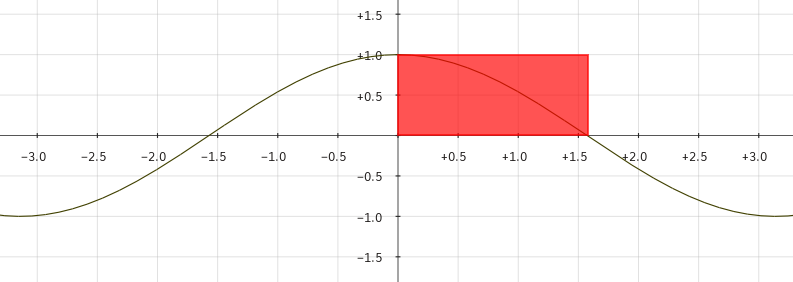
\includegraphics[width=0.8\textwidth]{img/coseno.png}
\caption{Comportamiento de la función $\cos$. En rojo la región que involucra los resutlados de la función de similitud}
\label{bus:img-coseno}
\end{figure}
El dominio de la función de similitud son los vectores normalizados con todas sus componentes mayores o iguales a 0.\\
\begin{figure}[H]
\centering
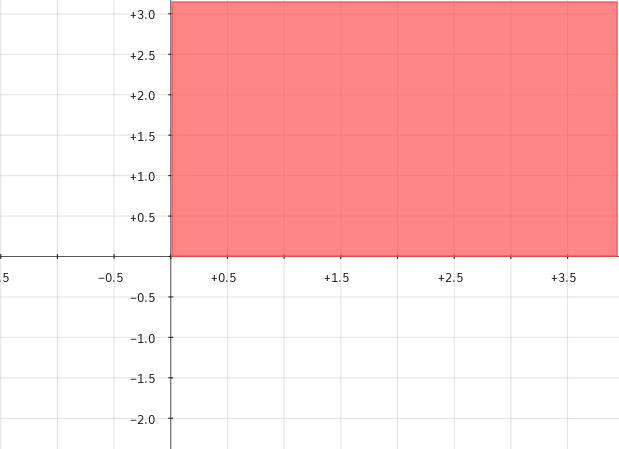
\includegraphics[width=0.4\textwidth]{img/planoCartesiano.png}
\caption{Plano cartesiano. En rojo al cuadrante al que pertenecen los vectores}
\label{bus:img-planoCartesiano}
\end{figure}
Del dominio de la función se obtiene que los ángulos que se forman se encuentran limitados entre $0$\textdegree y $90$\textdegree, 
o lo que es lo mismo $0$ y $\frac{\pi}{2}$. 
De lo anterior se obtien que:
$$0\leq \cos(\hat{\theta}) \leq 1$$
En el intervalo $[0, 1]$ la función $\cos$ es decreciente. Por lo que se definie la función de similitud como el $\cos$ del ángulo que forman de dos vectores. 
De esta manera los vectores tengan un ángulo cercano a $0$\textdegree son más similares. 

\section{Resolución}
Encontrar una solución al problema planteado es reducible 

El algoritmo que se utilizó para obtener las soluciones es \texttt{Produce-and-Choose}, cuenta con 
dos fases.
En la primer fase se generan cierta cantidad de bundles, e la fase siguiente se seleccionan los 
bundles que serán parte de la solución.\\
A continuación se explican los algoritmos utilizados para cada fase.
\section{Generación de bundles}
Dado un conjunto de papers el objetivo es generar clusters en los cuales los papers suficientemente 
similares pertenezcan al mismo cluster y en cluster distintos los disímiles. Cuanto mayor es la 
similitud en el cluster (intra) y mayor la diferencia entre los cluster (inter) es mejor la 
clusterización.\\
Definir como se constituye un cluster es complejo. Por ejemplo para los 20 puntos que se muestran a 
continuación existen tres (o más) formas de clusterizar que son validas. Entonces la mejor 
definición depende del tipo de dato y del resultado esperado.

\begin{figure}[H]
  \centering
    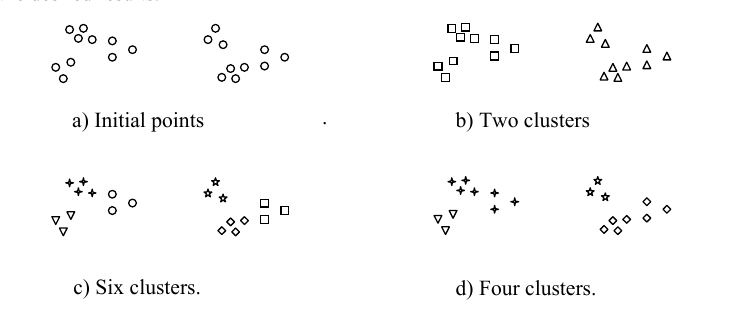
\includegraphics[width=0.8\textwidth]{img/howToCluster.png}
  \caption{Agregar descripcion}
  \label{res:img-howToCluster}
\end{figure}

En la clusterización para Composite Retrival, la definición es generar cluster máximizando el costo que esta acotado por el budget.
Ya que lo esperado es obtener cluster que utilicen el máximo del presupuesto.\\

El problema de la clusterización es NP-hard (agregar ref, explicar problema de clusterizacion),
por lo que se utilizaron dos técnicas ya conocidas para aproximarse a una solución.\\
La principal diferencia entre las estrategias de clusterización es entre la jerárquica y de 
partición.\\
La primer técnica produce un árbol de particiones, la raíz es un cluster que contiene todos los items
y las hojas son clusters con un único ítem. Cada nivel intermedio, puede ser visto, como la 
combinación entre dos clusters del nivel inferior inmediato. Mientras que la segunda genera solo un 
nivel de las particiones de los items de una vez.\\ 
Se implementaron las dos técnicas para la clusterización jerárquica con el algoritmo
Hierarchical clustering y la de partición con Bundles One-By-One.\\

\subsection{Bundles One-By-One}
El método \texttt{BOBO-x} esta inspirado en k-nn. Consiste en cada paso seleccionar, de manera azarosa, un item del conjunto de pivotes (en el inicio este conjunto contiente todos los items),
con el que se genera un bundle valido a al rededor de este. En el caso de que el intra del bundle sea bueno se agrga al conjunto de candidatos de bundle.
La iteración finaliza cuando se generan la cantidad de candidatos definidos en el parámetro $x$ o cuando el conjunto de bundles es vacío. El caso de que $x$ sea 'Ex' todos los 
items son pivotes.\\
Para generar el bundle a partir del pivote, se realiza de manera golosa de eligiendo en cada iteración el item que
máximiza el intra y que cumple con las resticciones.\\
\subsection{Hierarchical clustering}
La heurística Hierarchical clustering \texttt{HAC} comienza con tantos clusters como cantidad de elementos, cada uno está 
conformado por un solo ítem y en cada paso se unen los dos clusters más cercanos que respetan las restricciones. 
Para ello se define la función de distancia para los items $u$ y $v$ como:\\
\begin{equation}
d_{1}(u,v) = 1 - s(u, v)
\end{equation}

Con la función de distancia $d_{1}$ en la clusterización se generan los cluster lo más cohesivos posibles,
En la figura 1 se observa que el algoritmo selecciona los items más cercanos. En las búsquedas que 
se realizan en ``Composite ...''\cite{compositeRetrival} se tiene el parámetro $\gamma$ que indica 
que tipo de resultado es el esperado. 

\begin{figure}[H]
  \centering
    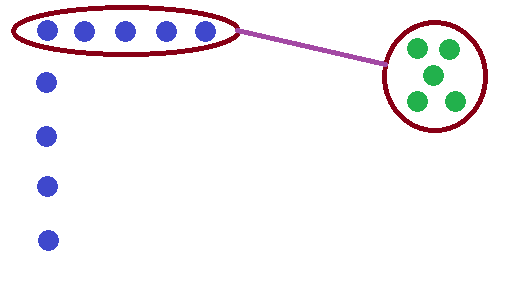
\includegraphics[width=0.3\textwidth]{img/cluster2.png}
  \caption{Selección de bundles usando $d_{1}$}
  \label{res:img-usingEfficientHAC}
\end{figure}

En caso de que el $\gamma$ sea pequeño, la 
clusterización esperada para la misma instancia es la que se visualiza en la imágen 2, clusters no 
tan cohesivos pero más variados. Por lo que se define una función de distancia que considera el 
$\gamma$.\\
\begin{equation}
d2(u,v) = 1 - FO(\{u\} \cup \{v\})
\end{equation}
Donde $FO$ es la función definida en \eqref{eq:fnObj} \\

\begin{figure}[H]
  \centering
    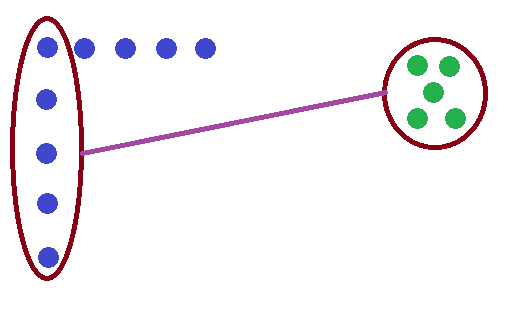
\includegraphics[width=0.3\textwidth]{img/cluster1.png}
  \caption{Selección de bundles usando $d_{2}$}
  \label{res:img-usingSingleHAC}
\end{figure}

Para la distancia $d_{1}$ se implementó el algoritmo \texttt{EfficientHAC} que es tiene una 
complejidad $\mathcal{O}(n^{2})$, mientras que para $d_{2}$ el algoritmo es \texttt{SingleHAC} que 
la complejidad es $\mathcal{O}(n^{2} * \ln{n})$. Según se demostró en el capítulo 17 de 
\cite{informationRetrival}


\section{Selección de bundles}
Al finalizar la producción de bundles, se deben seleccionar los $k$ bundles para la solución.
El problema de seleccionar los bundles que maximizan la función objetivo, se traduce en 
encontrar en el grafo G el k-subgrafo de mayor peso de nodos y aristas.

Se implementó el algoritmo que propone ``Composite ...''\cite{compositeRetrival} que transforma el 
grafo G en el grafo G', con los mismos nodos y aristas, redefiniendo el peso de las aristas con la 
función:\\

\begin{equation}
\omega_{1}(u,v) = \dfrac{\gamma}{2( k - 1)} (\omega(u) + \omega(v)) + (1 - \gamma)\psi(u,v) 
\end{equation}

(aca va el algoritmo)\\

En la función $\omega_{1}(u,v)$ el valor de la función $\psi(u,v)$  es considerablemente menor al de
$\omega(u) + \omega(v)$, (en el intra se suma los ejes de todos los nodos, el inter es el máximo entre los items)
implica que $\gamma$ no cumple con el objetivo de balancear entre una solución cohesiva y una variada.
Para esto se funciones $\omega$ alternativas.\\

Con $\omega_{2}(u,v,w,y)$ la búsqueda se realiza con la combinación de cuatro nodos, por lo que el orden de complejidad
aumenta a ...

\begin{equation}
\begin{split}
\omega_{2}(u,v,w,y) &= \dfrac{\gamma}{2( k - 1)} (\omega(u) + \omega(v) + \omega(w) + \omega(y)) \\
&+ (1 - \gamma)(\psi(u,v) + \psi(u,w) + \psi(u,y)  + \psi(v,w) + \psi(v,y) + \psi(w,y))
\end{split}
\end{equation}

La función $\omega_{3}(u, k)$ recibe $u$ el conjunto de clusters seleccionados hasta el momento 
y $k$ que es la cantidad de clusters para la solución. Con $k$ y el tamaño de $u$ se calcula el 
coeficiente con el propósito en que en cada paso se pondere el inter y el intra. Para eso se multiplica
con coeficientes cada parte de la función. Con esto se mantiene la relación de inter e intra durante la selección de bundles

\begin{equation}
\begin{split}
\omega_{3}(u,k) &= \dfrac{k}{u.size} * (\gamma \sum_{v \in U}(w(v))) \\
&+ \dfrac{(k * (k-1))}{2} * \dfrac{2}{(u.size() * (u.size() - 1))} * 1 - \gamma \sum_{v,w \in U}(\psi(v,w))
\end{split}
\end{equation}

\begin{algorithm}[H]
\begin{algorithmic}[1]
\REQUIRE $produced:Vector<SnowFlake>, numRequested:Integer$
\ENSURE $selected:Vector<SnowFlake>$.
\STATE $selected:Vector<SnowFlake> \leftarrow []$
\STATE $originalSize:Integer \leftarrow produced.size$
\WHILE {$selected.size < numRequested\ AND\ selected.size < originalSize$}
\STATE $selectedTemp \leftarrow selected$
\STATE $(candidateOne, candidateTwo) \leftarrow (i, j)\ where$ \\ 
$\displaystyle\max_{i \neq j} (FO(selectedTemp.push(produced_{i} \cup produced_{j})))$
\STATE $produced.erase(i)$
\STATE $produced.erase(j)$
\STATE $selected.push(candidateOne)$
\STATE $selected.push(candidateTwo)$
\ENDWHILE
\RETURN $selected$
\end{algorithmic}
\caption{Selección de bundles de a pares}\label{alg:algSelTuple}
\end{algorithm}
\subsection{Selección proporcional}
Además como tercera opción de selección se implementó un algoritmo proporcional que en cada paso se 
ponderan los resultados de la función que calcula el intra y el inter restante, intentando 
\textquotedblleft adivinar\textquotedblright  el valor de las próximas iteraciones y de esta manera 
dar más importancia en los primeras iteraciones al valor del inter.
\begin{algorithm}[H]
\begin{algorithmic}[1]
\REQUIRE $produced:Vector<SnowFlake>, numRequested:Integer$
\ENSURE $selected:Vector<SnowFlake>$
\STATE $w(u) = \dfrac{k}{u.size} * (\gamma \sum_{v \in U}(w(v))) + \dfrac{(k * (k-1))}{2} * \dfrac{2}{(u.size() * (u.size() - 1))} * 1 - \gamma \sum_{v,w \in U}(\psi(v,w))$
\STATE $available \leftarrow produced$
\STATE $selected \leftarrow []$
\WHILE {$selected.size < numRequested\ AND\ selected.size < produced.size$}
\STATE $candidate \leftarrow max_{i}$
\ENDWHILE
\RETURN $selected$
\end{algorithmic}
\caption{Selección de bundles proporcional}\label{alg:algSelProp}
\end{algorithm}

\section{Modificación de PAC para búsquedas específicas}
Para la obtención de la solución se modificó la producción de bundles como así también la 
selección de los mismos (Produce and Choose). \\
En la producción de bundles en el algoritmo jerárquico, se utilizó la similitud del perfil 
específico con los papers en cada paso que intenta unificar dos clusters. A diferencia del cálculo 
original que la compatibilidad de dos nodos esta dada por su distancia previamente obtenida, en 
este nuevo caso se agrega a ese resultado la compatibilidad de cada uno de ellos con el perfil 
específico. \\
Para la producción del algoritmo BOBO, se agregó junto al pivote en todos los clusters. \\
Para la selección de los bundles que formarán parte de la solución, a cada cluster se le 
calculo el valor intra también se tuvo en cuenta la similitud de todos los elementos con el perfil  
específico, de esta manera a los clusters que contenían papers con los mismos tópicos que el del 
vector especifico se le dio mayor peso.

\section{Heurística golosa para la obtención de una solución}
En todas los algoritmos previos se centraron en, primero construir buenos bundles maximizando solo 
el valor propio de cada bundle, o sea, el valor inter bundle. Una vez generado los suficientes 
\textquotedblleft buenos\textquotedblright  para luego seleccionar dependiendo de la 
estrategia elegida la solución final, ahora si, maximizando la función objetivo propuesta 
originalmente.\\
Para este heurística golosa propusimos ir construyendo los bundles finales teniendo en cuenta en 
cada paso la función objetivo, esto es, en cada paso cuando se intenta agregar un nuevo elemento a 
un bundle se calcula su valor total de la función y se evalúa en que bundle conviene agregarlo. 
Esto se repite para todos los items, haciendo que cuando tengo que agregar un nuevo ítem a la 
solución ya calculé para todos los items que no se encuentran en la solución en que bundle conviene 
agregarlo y cual es el valor de la función en ese caso, quedándonos siempre con el mejor valor 
posible.
\begin{algorithm}[H]
\begin{algorithmic}[1]
\REQUIRE $numOfSnowFlakes:Integer$
\ENSURE $selected:Vector<SnowFlake>$
\STATE $selected_{i}:Vector<SnowFlake> \leftarrow \emptyset_{0\leq i<numOfSnowFlakes}$
\STATE $isComplete:Bool \leftarrow False$
\STATE $elements:Set<Element> \leftarrow ElementsOfTheProblem$
\WHILE {$isComplete == False$}
\STATE $bestScore:Double \leftarrow -\infty$
\STATE $bestElement:Element \leftarrow \varnothing$
\STATE $bestBundle:SnowFlake \leftarrow \varnothing$
\FOR {$elem:Element \in elements$}
\FOR {$bundle:SnowFlake \in selected$}
\IF {$isValidBundle(bundle \cup \{elem\}) == True$}
\STATE $score:Double \leftarrow FO(selected.replace(bundle, bundle \cup \{elem\}))$
\IF {$score > bestScore$}
\STATE $bestScore \leftarrow score$
\STATE $bestBundle \leftarrow bundle$
\STATE $bestElement \leftarrow elem$
\ENDIF
\ENDIF
\ENDFOR
\ENDFOR
\STATE $selected \leftarrow selected.replace(bundle, bundle \cup \{elem\})$
\STATE $elements.erase(elem)$
\STATE $isComplete \leftarrow bestElement == \varnothing$
\ENDWHILE
\RETURN $selected$
\end{algorithmic}
\caption{Algoritmo heurística golosa}\label{alg:algHeuGol}
\end{algorithm}

\chapter{Experimentación computacional}
\label{chap:experimentacion}
\section{Instancias de pruebas}\label{sect:busquedas}
En esta sección se presentan las consultas utilizadas para evaluar las propuestas algorítmicas introducidas en este trabajo. 

Las consultas se hicieron sobre dos bases de datos. Una de ellas, corresponde a la base de datos de artículos provista por \textit{\textquotedblleft A Data-Driven Journey through Software Engineering Research\textquotedblright}\cite{dataDrive}. La otra corresponde a atracciones turísticas de Europa obtenida de las pruebas realizadas en \cite{journals/tkde/Amer-YahiaBCFMZ14}.

A continuación se describe para cada consulta, realizada sobre las bases de datos, la función de similitud, el atributo utilizado para definir la complementariedad de los elementos y el presupuesto elegidos para las instancias escogidas. 

Para la experimentación se utilizó una máquina Desktop Intel(R) Core(TM) i5-4570T CPU @ 2.90GHz, 5.7G Ram, con DB: 5.5.46-MariaDB-1ubuntu0.14.04.2.

\subsection{Base de datos de artículos}
La base de datos utilizada es la proporcionada por \textit{\textquotedblleft A Data-Driven Journey through Software Engineering Research\textquotedblright}\cite{dataDrive}. La misma contiene unos $7800$ artículos relacionados con la Ingeniería de Software presentados en diferentes conferencias entre los años 1975 y 2011. Los artículos se encuentran catalogados por autores, tópicos relevantes, conferencia donde fue presentado el trabajo y afiliaciones. Además los artículos están clasificados mediante \texttt{topicProfile}. La clasificación es asignada a cada artículo en base a las citas provenientes de otros trabajos publicados en conferencias específicas sobre alguno de los 37 tópicos que fueron tratados en \cite{dataDrive}. Como resultado, cada \texttt{topicProfile} expresa el porcentaje de relevancia de cada uno de los tópicos encontrados dentro del artículo. 

De los $9800$ autores contenidos en la base de datos, se tiene la información de la universidad a la que cada uno pertenece y la región donde se encuentra dicha universidad.

El \texttt{topicProfile} es lo que permitirá definir la similitud, no sólo entre los artículos, sino también entre los autores y las universidades de la base de datos, de una manera prácticamente directa.

Los criterios de las búsquedas realizadas sobre la base de datos se concibieron a partir de lo que se considera que es de interés general. Por ejemplo, una posible consulta sobre esta base de datos podría ser la búsqueda de artículos sobre núcleos temáticos característicos en las distintas conferencias, de manera que observando un paquete se podría conocer qué se dice sobre este tema en cada una de las conferencias. En otro escenario, con el propósito de armar paneles de expertos, puede resultar de interés la búsqueda de investigadores que trabajan en tópicos similares con afiliación en distintas universidades. También se puede querer conocer universidades de distintas regiones con grupos de investigación trabajando en tópicos similares.

Por lo establecido en \cite{journals/tkde/Amer-YahiaBCFMZ14} para las búsquedas se deben realizar las siguientes definiciones:
\begin{itemize}
  \item \textbf{Similitud}: Función que dado dos ítems devuelve la similitud entre estos.
  \item \textbf{Costo}: Función que dado un ítem devuelve el costo del mismo.
  \item \textbf{Presupuesto}: El presupuesto que se tiene, el cual no podrá ser excedido por ningún paquete.
  \item \textbf{Complementariedad}: Propiedad del ítem que es único en cada paquete.
\end{itemize}

Para todas las búsquedas, sin importar el ítem que sea (artículo, autor o universidad), se definió que el costo de cada ítem sea de una unidad y que el presupuesto para cada búsqueda sea de cinco unidades. En consecuencia, todos los paquetes de todos los resultados contienen como máximo cinco ítems. Se tomó esta decisión para que cada paquete contenga como máximo un número fijo de elementos. Además se estableció que sean diez los paquetes devueltos en cada búsqueda. El motivo para tomar esta decisión es que un humano pueda valorizar el resultado propuesto fácilmente. Entonces, de aquí en adelante, para cada criterio de búsqueda se deben definir únicamente la función de similitud y la propiedad de complementariedad.

El \texttt{Topic Profile} define el perfil de un artículo asignándole un porcentaje a cada tópico que se hace referencia. En el caso del artículo \texttt{A Cognitive-Based Mechanism for Constructing Software Inspection Teams} el \texttt{Topic Profile} se compone por los tópicos  REQUIREMENTS, RELIABILITY, TESTING y SOFTWARE QUALITY. El porcentaje de cada uno de estos es 71.43 \%, 17.86 \%, 7.14 \% y 3.57 \% respectivamente. Esto significa que el 71.43\% de los trabajos citados en este artículo fueron presentados en conferencias o publicados en revistas vinculadas al área REQUIREMENTS.

El modelo computacional del perfil de cada artículo es un vector cuya dimensión corresponde a la cantidad de tópicos y cada posición representa un tópico diferente. El valor de cada posición del vector es el porcentaje del tópico que le corresponde a ese artículo según el \textit{Topic Profile} de la base de datos. Más adelante se explica cómo estos vectores se utilizan para comparar la similitud entre los artículos.

Para los autores no se cuenta con información más allá de los artículos que escribieron, pero sólo con eso alcanza para poder generar un perfil de autores. Para cada autor se hace la suma vectorial de cada uno de los \texttt{Topic Profile} de los artículos en los cuales participó y con eso se obtiene el \texttt{Topic Profile de Autores}. Para obtener el perfil de las universidades se aplicó el mismo criterio. Se realiza la suma vectorial de cada uno de los \texttt{Topic Profile de Autores} pertenecientes a la misma universidad y así se genera el \texttt{Topic Profile de Universidades}. En ambos casos se aplica la normalización sobre los vectores resultantes.

Para clarificar se presenta un ejemplo de los perfiles de los elementos:

\begin{table}[H]
\begin{tabular}{lll}
	Artículo & Topic Profile & Autores \\
	Artículo 1 & $[$0.20, 0.40, 0.40, 0.00$]$ & Autor 1, Autor 2, Autor 3 \\
	Artículo 2 & $[$0.30, 0.70, 0.00, 0.00$]$ & Autor 2, Autor 3 \\
	Artículo 3 & $[$0.00, 0.10, 0.00, 0.90$]$ & Autor 2 \\
	Artículo 4 & $[$0.00, 0.00, 1.00, 0.00$]$ & Autor 1, Autor 3 \\
\end{tabular}
\label{tabla:topicProfileEj1}
\end{table}

\begin{table}[H]
\begin{tabular}{lll}
	Autor & Topic Profile & Universidad \\
	Autor 1 & $[$0.14, 0.27, 0.95, 0.00$]$ & Universidad 1 \\
	Autor 2 & $[$0.30, 0.74, 0.25, 0.55$]$ & Universidad 2 \\
	Autor 3 & $[$0.27, 0.60, 0.76, 0.0$]$ & Universidad 2 \\
\end{tabular}
\label{tabla:topicProfileEj2}
\end{table}

\begin{table}[H]
\begin{tabular}{ll}
	Universidad & Topic Profile \\
	Universidad 1 & $[$0.14, 0.27, 0.95, 0.00$]$ \\
	Universidad 2 & $[$0.31, 0.72, 0.54, 0.30$]$ \\
\end{tabular}
\label{tabla:topicProfileEj3}
\end{table}

Para la evaluación de los algoritmos propuestos en esta tesis, se realizaron las siguientes consultas:
\begin{enumerate}
	\item
		Artículos con tópicos similares presentados en distintas conferencias. \label{busqueda:articulos}
		\begin{itemize}
			\item \textbf{Similitud}: Función que compara el perfil de cada artículo.
			\item \textbf{Complementariedad}: Lugar dónde fue presentado.
		\end{itemize}

	\item
	Autores que escribieron artículos con tópicos similares afiliados a universidades distintas. \label{busqueda:autores}
	\begin{itemize}
		\item \textbf{Similitud}: Función que compara el perfil de los autores.
		\item \textbf{Complementariedad}: Universidad de pertenencia del autor.
	\end{itemize}

	\item 
	Universidades en donde se escribieron artículos de tópicos similares que se encuentran en distintas regiones. \label{busqueda:universidades}
	\begin{itemize}
		\item \textbf{Similitud}: Función que compara el perfil de las universidades.
		\item \textbf{Complementariedad}: Región de la institución.
	\end{itemize}
\end {enumerate}

Para obtener resultados de mayor calidad, se depuró de la base de datos aquellos artículos que no contengan la información del autor, de los tópicos (\textbf{topic profile}) o del lugar de publicación (\textbf{venue}). Quedando, luego de la depuración, $5500$ artículos.  

\paragraph{Función de similitud}
La similitud se emplea para comparar dos objetos y determinar qué tan parecidos son entre sí. En este trabajo se definió la similitud entre los objetos de la base de datos de artículos mediante la \textbf{similitud coseno}. Esta es una medida de similitud entre dos vectores en un espacio vectorial provisto de un producto escalar que mide el coseno del ángulo comprendido entre ellos.

Entonces se define la función de similitud $S(U_i, V_j)$ para los vectores $U_i$ y $V_j$ a partir del producto escalar

\begin{equation} \label{eq:angulovectorial}
\cos(\theta) =  \dfrac{\overrightarrow{U_i} \overrightarrow{V_j}}{\overrightarrow{\lVert U_i\lVert} \overrightarrow{\lVert V_j\lVert}}
\end{equation}

Para esta instancia los objetos (ahora artículos, autores o universidades) están representados por vectores, donde cada dimensión corresponde a un tópico cuyo valor se corresponde con el valor del tópico del objeto según la base de datos \cite{dataDrive}. Por lo tanto el objeto $a$ se representa con el vector $V_a = [v_1,v_2,...,v_3]$ que cumple con las siguientes propiedades:
\begin{enumerate}
 \item $v_i \geq 0$
 \item $\sum{v_i} = 1$
\end{enumerate}

Como los componentes de todos los vectores son mayor o igual a cero se obtiene que $0\leq\cos(\theta)\leq1$, que implica que $S(V_i, V_j) \in \left[0, 1\right]$.

\begin{figure}[H]
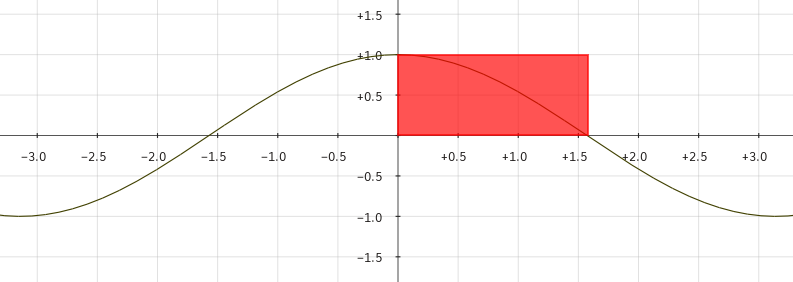
\includegraphics[width=0.8\textwidth]{img/coseno.png}
\caption{Comportamiento de la función $\cos$. En rojo la región que pertenece a la función de similitud}
\label{bus:img-coseno}
\end{figure}

%Para \textbf{similitud coseno} dos vectores proporcionales con la misma dirección la similitud es 1 (ya que es 0 el ángulo que se forma). Por lo que esta similitud no diferencia entre un artículo profesional y un artículo de un diario que cubre el mismo tópico. Por ejemplo si dos artículos que cubren un mismo y único tópico, pero para uno el valor del tópic Esta debilidad de la medida basada en el ángulo no interfiere en este trabajo por la segunda propiedad de los vectores del problema, porque para que dos vectores sean proporcionalmente iguales tienen que ser idénticos y en tal caso es correcto que la similitud entre ellos sea 1.

Con el objetivo de simplificar la ejecución de los algoritmos, considerando que el costo de calcular $cos()$ de los vectores es alto, se decidió realizar el cálculo de la similitud de los artículos, autores y universidades previamente a la ejecución de los algoritmos de búsquedas.

\subsection{Base de dato de atracciones turísticas}
Se utilizó una instancia de datos correspondiente a 200 atracciones turísticas de Europa, con datos relevados del sitio \textit{TripAdvisor}. De cada atracción se tiene la información del precio, del tipo (parque, museo, edificio) y de la distancia geográfica con el resto de las atracciones.

El propósito de la búsqueda es darle al usuario distintas opciones de circuitos turísticos que contienen atracciones, con los siguientes requerimientos: evitar realizar largos traslados, variedad en el tipo de atracción y que el costo del circuito no supere el presupuesto del turista. Por lo tanto el modelo de la búsqueda quedó diseñado de la siguiente manera: \label{busqueda:atracciones}

\begin{itemize}
	\item \textbf{Similitud}: La inversa de la distancia entre las atracciones. 
	\item \textbf{Costo}: Precio de la atracción. 
	\item \textbf{Presupuesto}: Presupuesto del turista. 
	\item \textbf{Complementariedad}: Tipo de atracción.
\end{itemize}

\section{Resultados}\label{sect:resultados}

En esta sección se analizarán los resultados computacionales comparando la calidad de las soluciones obtenidas por los algoritmos discutidos en \autoref{chap:nuevas-propuestas}, sobre las bases de datos de \autoref{sect:busquedas}. Con el objetivo de evaluar las propuestas algorítmicas, se consideraron los siguientes métodos.

\begin{itemize}
\item{$alg1$} PAC(C-HAC / selección simple)
\item{$alg2$} PAC(BOBO-10 / selección simple)
\item{$alg3$} PAC(BOBO-10 / selección proporcional)
\item{$alg4$} PAC(BOBO-10 / selección proporcional) + tabú
\item{$alg5$} PAC(Intra-Inter C-HAC / selección proporcional)
\item{$alg6$} PAC(Intra-Inter C-HAC / selección proporcional) + tabú
\item{$alg7$} Construcción golosa
\item{$alg8$} Construcción golosa + tabú
\end{itemize}

Tanto $alg1$ como $alg2$ corresponden a las metodologías propuestas en \cite{journals/tkde/Amer-YahiaBCFMZ14}. Los demás algoritmos involucran las mejoras propuestas en este trabajo. En \texttt{PAC}, la búsqueda tabú \texttt{Inter-Paquete} se realiza al finalizar la etapa de producción y la \texttt{Intra-Paquete} luego de la selección. En la \texttt{Búsqueda Golosa} se intenta mejorar la solución obtenida mediante la búsqueda tabú \texttt{Intra-Paquete}. Cabe señalar que no se tienen en consideración BOBO-Ex y CAP, ya que para el tamaño de la instancia los tiempos de ejecución de esos algoritmos resultaron prohibitivos. A partir de una experimentación preliminar con BOBO para valores $c=1, 5$ y $10$, resultó $c=10$ la opción más competitiva. Para la búsquedas tabú se definió que la cantidad de iteraciones de permanencia de un elemento en la lista tabú sea el promedio de elementos que tiene un paquete en la solución inicial.

Para realizar una comparación entre la calidad de las soluciones obtenidas por los diferentes algoritmos, se ha evaluado para los $\gamma \in \left\{0,1; 0,3; 0,4; 0,5; 0,6; 0,7; 0,8; 0,9\right\}$ el porcentaje de deterioro de cada solución respecto de la mejor solución obtenida por alguno de los ocho algoritmos.

En el caso de la búsqueda de artículos, que es el escenario que contiene la mayor cantidad de objetos, los tiempos de ejecución para los algoritmos C-HAC ($alg1$, $algo5$ y $alg6$), BOBO ($alg2$, $alg3$ y $alg4$) y los golosos ($alg7$ y $alg8$) son del orden de los 5, 2 y 6 minutos respectivamente. Los incrementos de tiempo debido a la ejecución de las metaheurísticas de mejora son despreciables, están entre los 5 y 7 segundos. Por lo cual no se considera que el tiempo sea un factor que valga la pena analizar.

\subsection{Análisis de los resultados obtenidos de la base de datos de artículos}
Para comprender el comportamiento de los resultados de las búsquedas se diseñaron dos tipos de gráficos que permiten visualizar la cohesión de los paquetes y la dispersión entre ellos. De esta forma se podrá analizar la calidad del resultado obtenido, más allá del valor de la función objetivo.

Los gráficos del estilo de la figura \ref{res:img-explain-bars} permiten analizar la distribución de los tópicos de una solución a nivel de paquete y de la relación con otros. Las filas corresponden a los 10 paquetes obtenidos y las columnas a los 37 tópicos considerados. El tamaño del círculo representa la proporción del tópico en el perfil del artículo y el color hace referencia al paquete al cual el artículo pertenece. Por lo tanto, dos artículos tendrán gran similitud cuando los patrones de sus círculos coincidan, tanto en tamaño como en distribución. Si para un paquete la distribución entre los tópicos y el tamaño de los círculos es similar entre sus artículos se puede deducir que este paquete es cohesivo (tiene buen valor intra). Por otro lado, si los patrones de los círculos de los dos artículos más similares entre distintos paquetes no coinciden, esto indica que el resultado es diverso.
\begin{figure}[H]
  \centering
    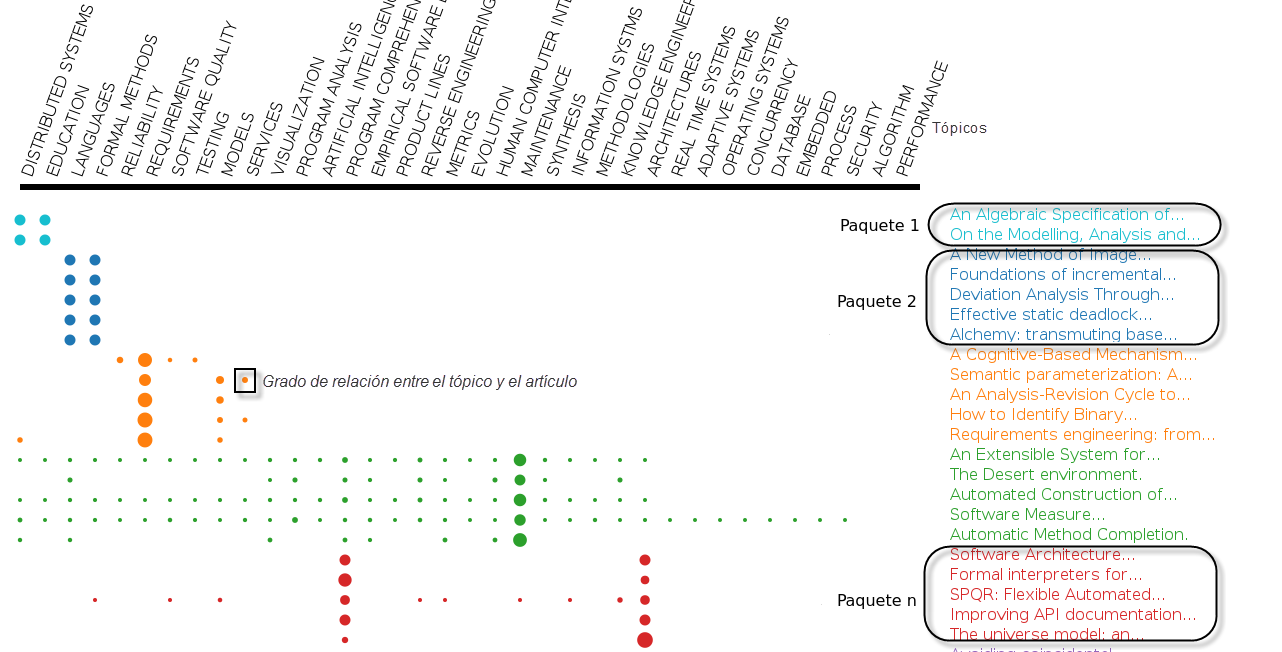
\includegraphics[width=1\textwidth]{img/explain-bars.png}
  \caption{}
  \label{res:img-explain-bars}
\end{figure}

Los gráficos de tipo burbuja de la figura \ref{res:img-explain-bubbles} son útiles para concluir el nivel de acoplamiento entre los paquetes de una solución, observando la relación entre los tópicos y los paquetes. Cada burbuja representa un tópico y cada círculo dentro de esa burbuja es un artículo. El tamaño del circulo es la proporción del artículo con el tópico y el color es el paquete al que pertenece. Entonces, si las burbujas contienen círculos de tamaños parecidos de más de un color se puede decir que ese resultado no es muy diverso. Por otro lado, mientras que el color de los círculos de las burbujas sea más homogéneo el resultado será más diverso. En cuanto a la cohesión de los paquetes, es más cohesivo cuando el tamaño de cada círculo dentro de las burbujas es similar (para el mismo color) y cada una de ellas contiene la misma cantidad, o ninguno, de círculos del mismo color.

\begin{figure}[H]
  \centering
    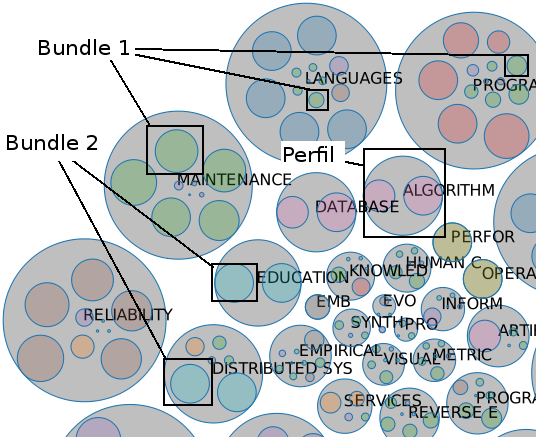
\includegraphics[width=0.5\textwidth]{img/explain-bubbles.png}
  \caption{}
  \label{res:img-explain-bubbles}
\end{figure}

\subsubsection{Búsqueda de artículos}
Para la búsqueda de artículos con tópicos similares en la tabla \ref{tabla:comp1} se observa los porcentajes de deterioro de cada solución respecto de la mejor solución obtenida por alguno de los ocho algoritmos. Una primera observación es que los algoritmos  Intra-Inter C-HAC reflejan el efecto buscado: a menores valores de $\gamma$ donde el valor inter tiene mayor peso, se obtienen mejores soluciones. Es decir, haber considerado en el proceso de generación de paquetes la función Intra-Inter benefició a la calidad de las soluciones obtenidas. Los algoritmos BOBO, no obtuvieron soluciones de la calidad de los algoritmos C-HAC y el proceso de selección proporcional no logró una mejora consistente para todos los valores de $\gamma$. Las soluciones obtenidas con el algoritmo de construcción golosa, no alcanzaron a mejorar las soluciones de C-HAC pero fueron ampliamente mejores que las de BOBO. En promedio el porcentaje de deterioro de BOBO fue de un $50\%$ mientras que el goloso fue de un $12\%$. 

Cabe resaltar el muy buen rendimiento de la búsqueda tabú, tanto en escenarios donde la solución inicial no es de buena calidad (algoritmo BOBO) así como también considerando soluciones de mejor calidad (algoritmo Intra-Inter C-HAC). En el primer caso, se obtienen porcentajes de mejora por encima del $70\%$. En el segundo caso, para varios valores de $\gamma$ la solución obtenida por la búsqueda tabú resultó ser la mejor opción y en otros con deterioros inferiores al $0.5\%$.

Si bien el algoritmo goloso no alcanzó los valores obtenidos por las soluciones generadas por C-HAC, tiene como ventaja su fácil y rápida implementación. Sus tiempos de ejecución fueron levemente mayores a los que se obtuvieron con BOBO y menores a las ejecutadas por C-HAC. Por la forma en la que fue construido siempre genera paquetes completos. Si bien la definición formal del problema no obliga a esto último, se implementó de esta manera ya que a efectos de un usuario final es más interesante obtener paquetes completos, aunque esto signifique sacrificar la búsqueda de la solución óptima.

\begin{table}[H]
\begin{center}
\begin{tabular}{|c|c|c|c|c|c|c|c|c|}
\hline
$\gamma$&$alg1$&$alg2$&$alg3$&$alg4$&$alg5$&$alg6$&$alg7$&$alg8$ \\ \hline
0.1 & -2.05 & -32.70 & -36.18 & -7.45 & -0.42 & 0.00 & -4.53 & -3.53 \\
0.2 & -2.11 & -38.06 & -41.19 & -8.23 & 0.00 & 0.00 & -4.92 & -3.85 \\
0.3 & -2.31 & -45.21 & -47.35 & -8.01 & 0.00 & 0.00 & -9.17 & -7.66 \\
0.4 & -0.14 & -49.08 & -51.22 & -15.51 & 0.00 & 0.00 & -10.40 & -9.35 \\
0.5 & 0.00 & -52.35 & -54.23 & -17.87 & -0.31 & -0.31 & -12.97 & -10.38 \\
0.6 & 0.00 & -55.16 & -56.04 & -14.43 & -0.05 & -0.05 & -14.78 & -13.69 \\
0.7 & 0.00 & -56.88 & -56.57 & -17.02 & -0.41 & -0.41 & -16.21 & -15.08 \\
0.8 & 0.00 & -57.86 & -57.86 & -16.11 & -0.56 & -0.30 & -18.10 & -17.60 \\
0.9 & 0.00 & -58.92 & -58.92 & -15.91 & -0.48 & -0.35 & -20.47 & -17.61 \\ \hline 
\end{tabular}
\caption{Comparación de calidad de soluciones entre algoritmos para la \hyperref[busqueda:articulos]{búsqueda de artículos}} 
\label{tabla:comp1}
\end{center}
\end{table}

Para comprender la semántica de las soluciones se compararon las soluciones con $\gamma = 0,1$ y $\gamma = 0,9$. En la figura \ref{res:comp1} se observa que para $\gamma = 0,1$ los tópicos (representados por burbujas) para la solución de \textit{alg 3} están presentes en varios paquetes (representados por círculos de colores). En cambio en el $alg6$ la mayoría de las burbujas contiene círculos de un solo color. De esta manera se visualiza que la solución de $alg6$ es más diversa. En $\gamma = 0,9$ el resultado obtenido con $alg3$ no se visualiza que cada burbuja contenga cinco círculos del mismo color, en cambio si sucede para la solución de $alg1$. Eso significa que los paquetes de la solución de $alg1$ son más cohesivos, ya que los cinco elementos de cada paquete tienen los mismos tópicos.

\begin{figure}[H]
	\centering
	\begin{tabular}{cc}
		\multicolumn{2}{c}{$\gamma=0.1$}\vspace{0.5cm}\\
		$alg3$ & $alg6$\\
		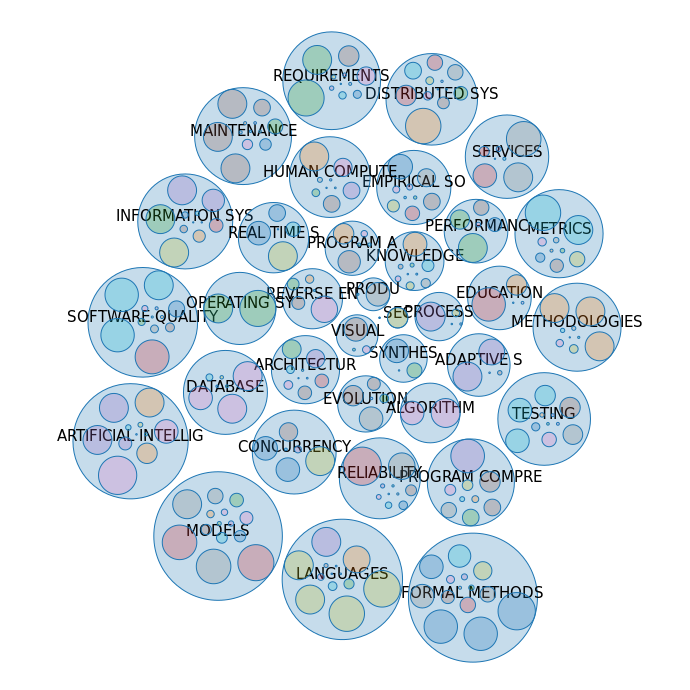
\includegraphics[width=0.45\linewidth]{img/gamma-01-burbujas-alg-3.png}&
		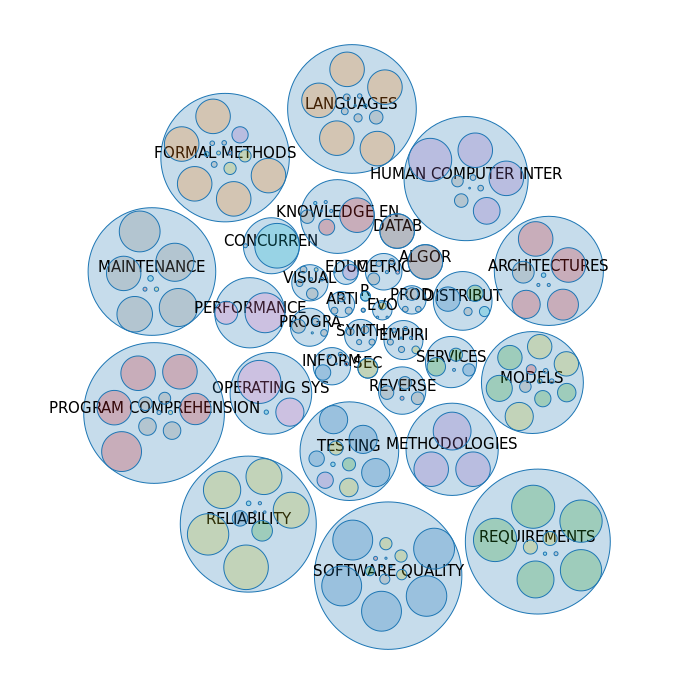
\includegraphics[width=0.45\linewidth]{img/gamma-01-burbujas-alg-6.png}\vspace{1cm}\\
		\multicolumn{2}{c}{$\gamma=0.9$}\vspace{0.5cm}\\
		$alg3$ & $alg1$\\
		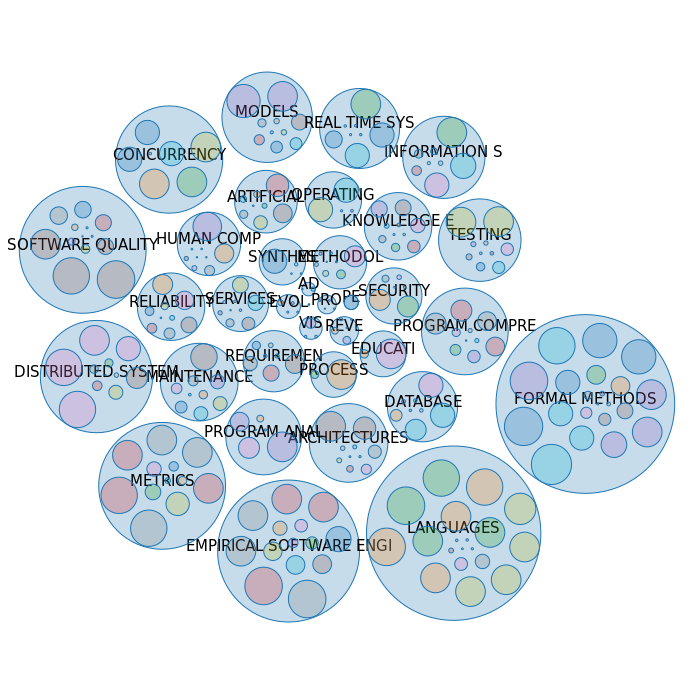
\includegraphics[width=0.45\linewidth]{img/gamma-09-burbujas-alg-3.png}&
		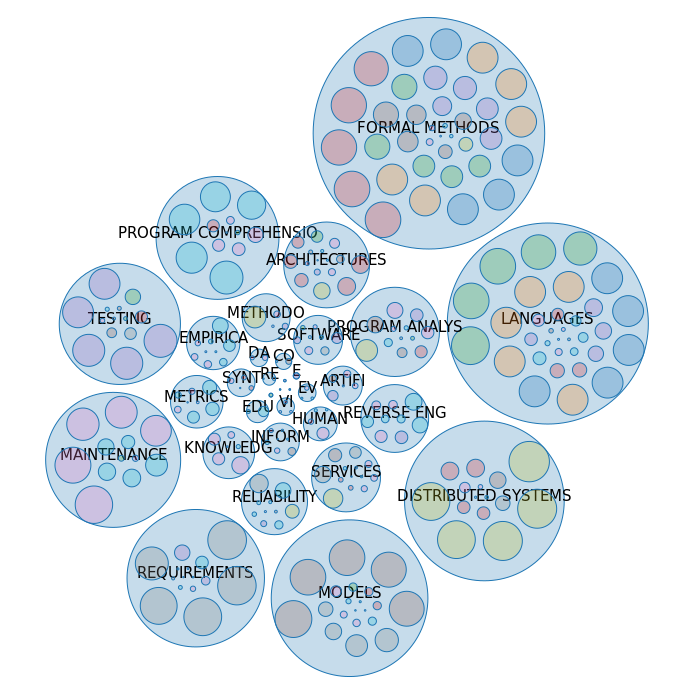
\includegraphics[width=0.45\linewidth]{img/gamma-09-burbujas-alg-1.png}\\
	\end{tabular}
	\caption{Comparación entre las soluciones con menor(izq) y mayor(der) función objetivos  para $\gamma\ =\ 0,1\ y \gamma\ =\ 0,9$}
	\label{res:comp1}
\end{figure}

La búsqueda tabú tiene su mayor impacto cuando es aplicada a la solución brindada por el algoritmo $alg3$, como puede observarse en la tabla \autoref{tabla:comp1} y en este contexto resulta una buena alternativa por su bajo costo computacional. En la Figura~\ref{res:bobo} se observa que para $\gamma=0.1$, la solución dada por el $alg3$ tiene artículos de distintos paquetes con patrones muy similares indicando un bajo valor inter-paquete. Por el contrario, luego de aplicar la búsqueda tabú los patrones de los artículos más similares entre distintos paquetes se volvieron más dispares, demostrando el aumento de la diversidad entre paquetes. Para $\gamma=0.9$, como puede observarse en la misma Figura~\ref{res:bobo}, en la solución brindada por el $alg4$ todos los paquetes tienen al menos un artículo cuyo patrón consiste en muchos círculos pequeños distribuidos en la mayoría de los tópicos en contraposición al resto de los artículos del mismo paquete con pocos círculos de gran tamaño. Demostrando un bajo valor intra-paquete. En contraposición a los paquetes obtenidos luego de aplicar la búsqueda tabú, los cuáles son mucho más cohesivos. La última afirmación puede observarse en los círculos de los artículos dentro de un mismo paquete, quienes siguen patrones mucho más parecidos. Se puede afirmar que la búsqueda tabú es capaz de mejorar las características de la solución en función del parámetro $\gamma$.

\begin{figure}[H]
	\centering
	\begin{tabular}{cc}
		$alg3$ & $alg4$\vspace{0.5cm}\\
		\multicolumn{2}{c}{$\gamma=0.1$}\\
		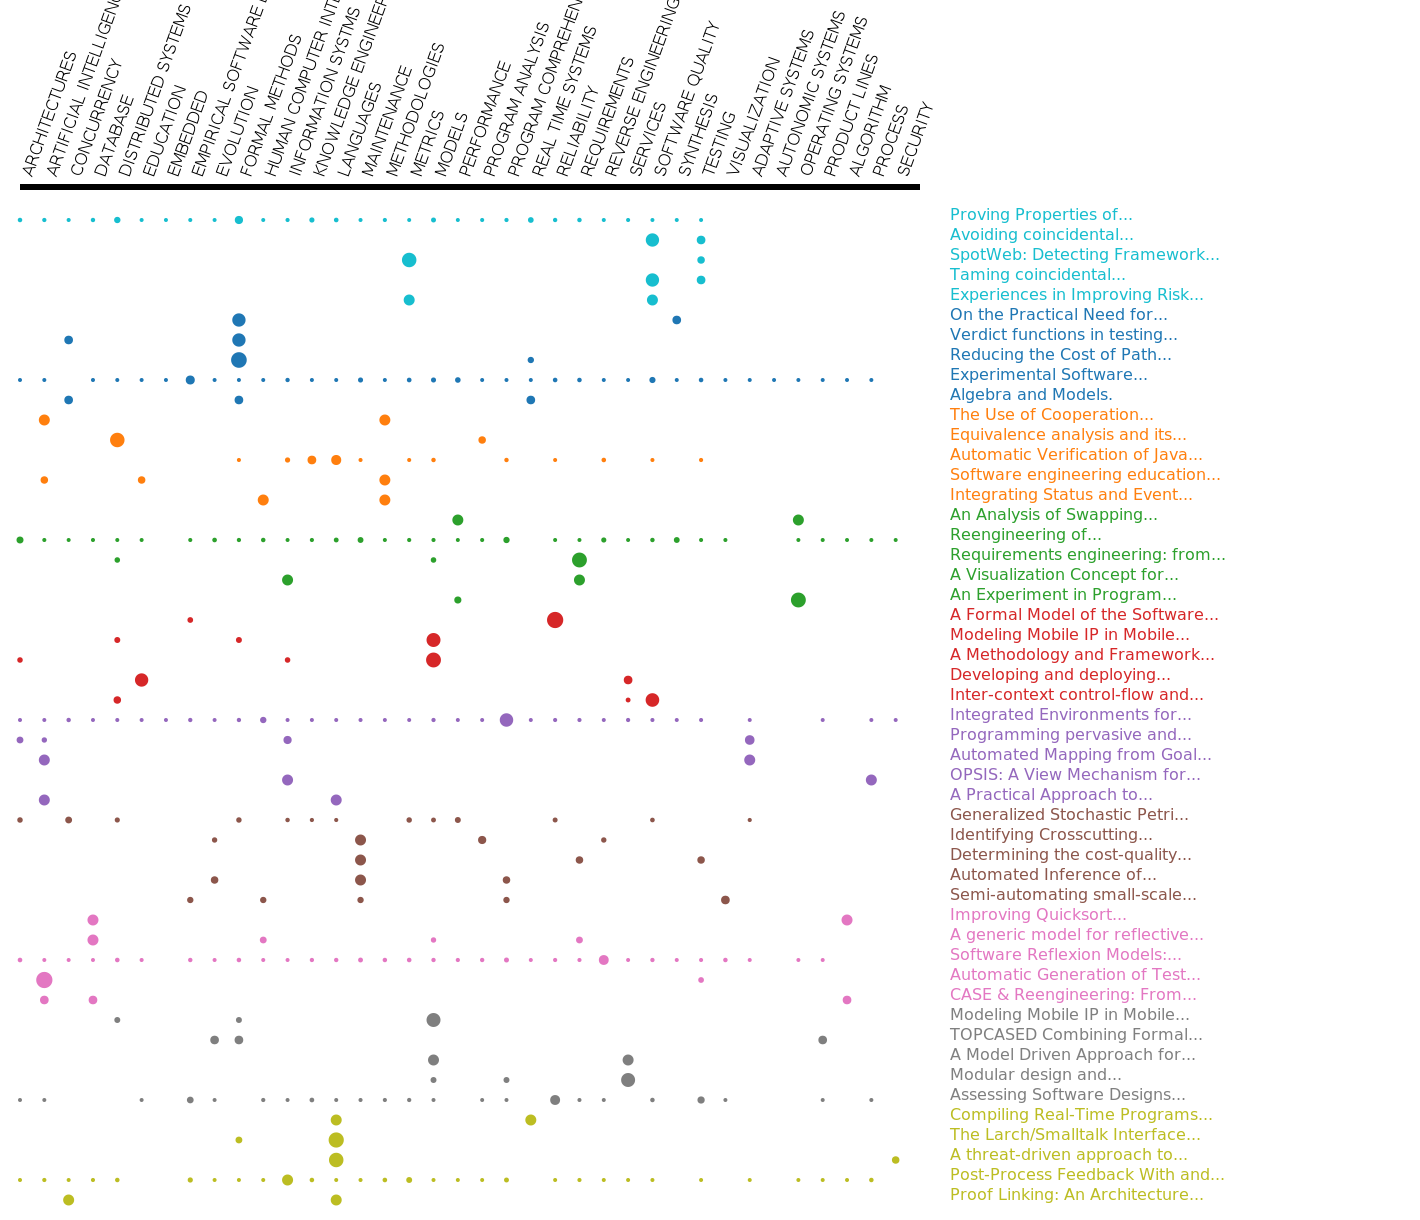
\includegraphics[width=0.45\linewidth]{img/gamma-01-alg-3.png}&
		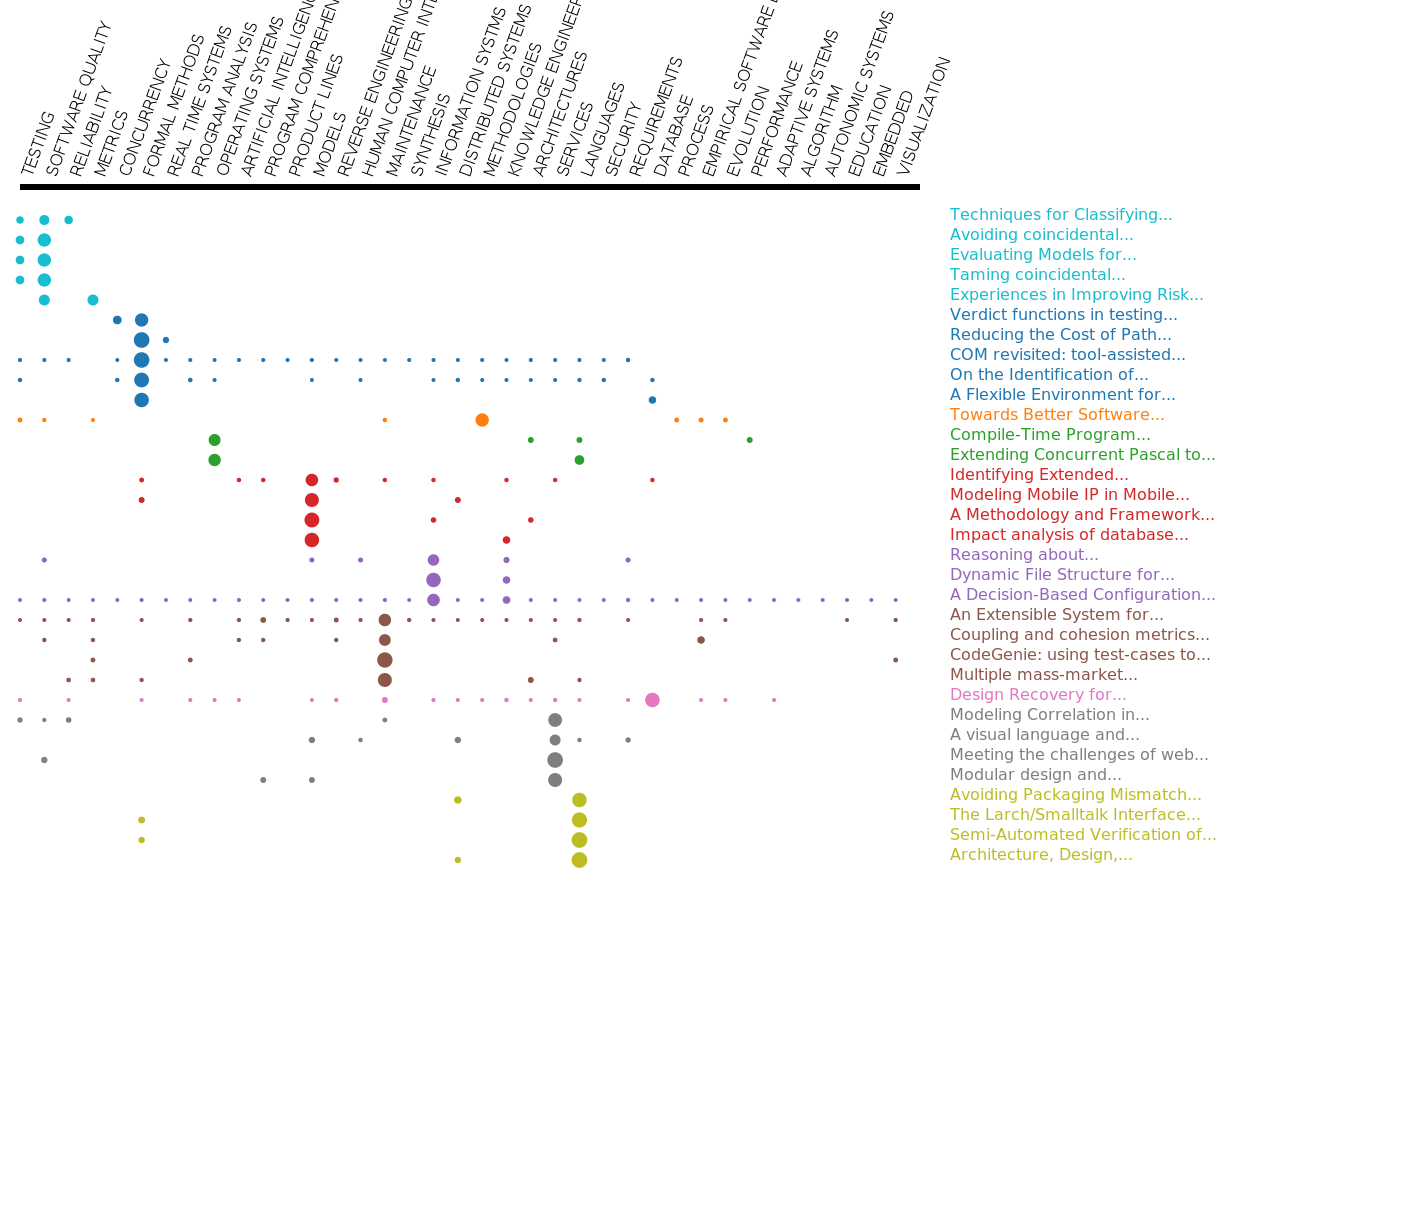
\includegraphics[width=0.45\linewidth]{img/gamma-01-alg-4.png}\vspace{1cm}\\
		\multicolumn{2}{c}{$\gamma=0.9$}\\
		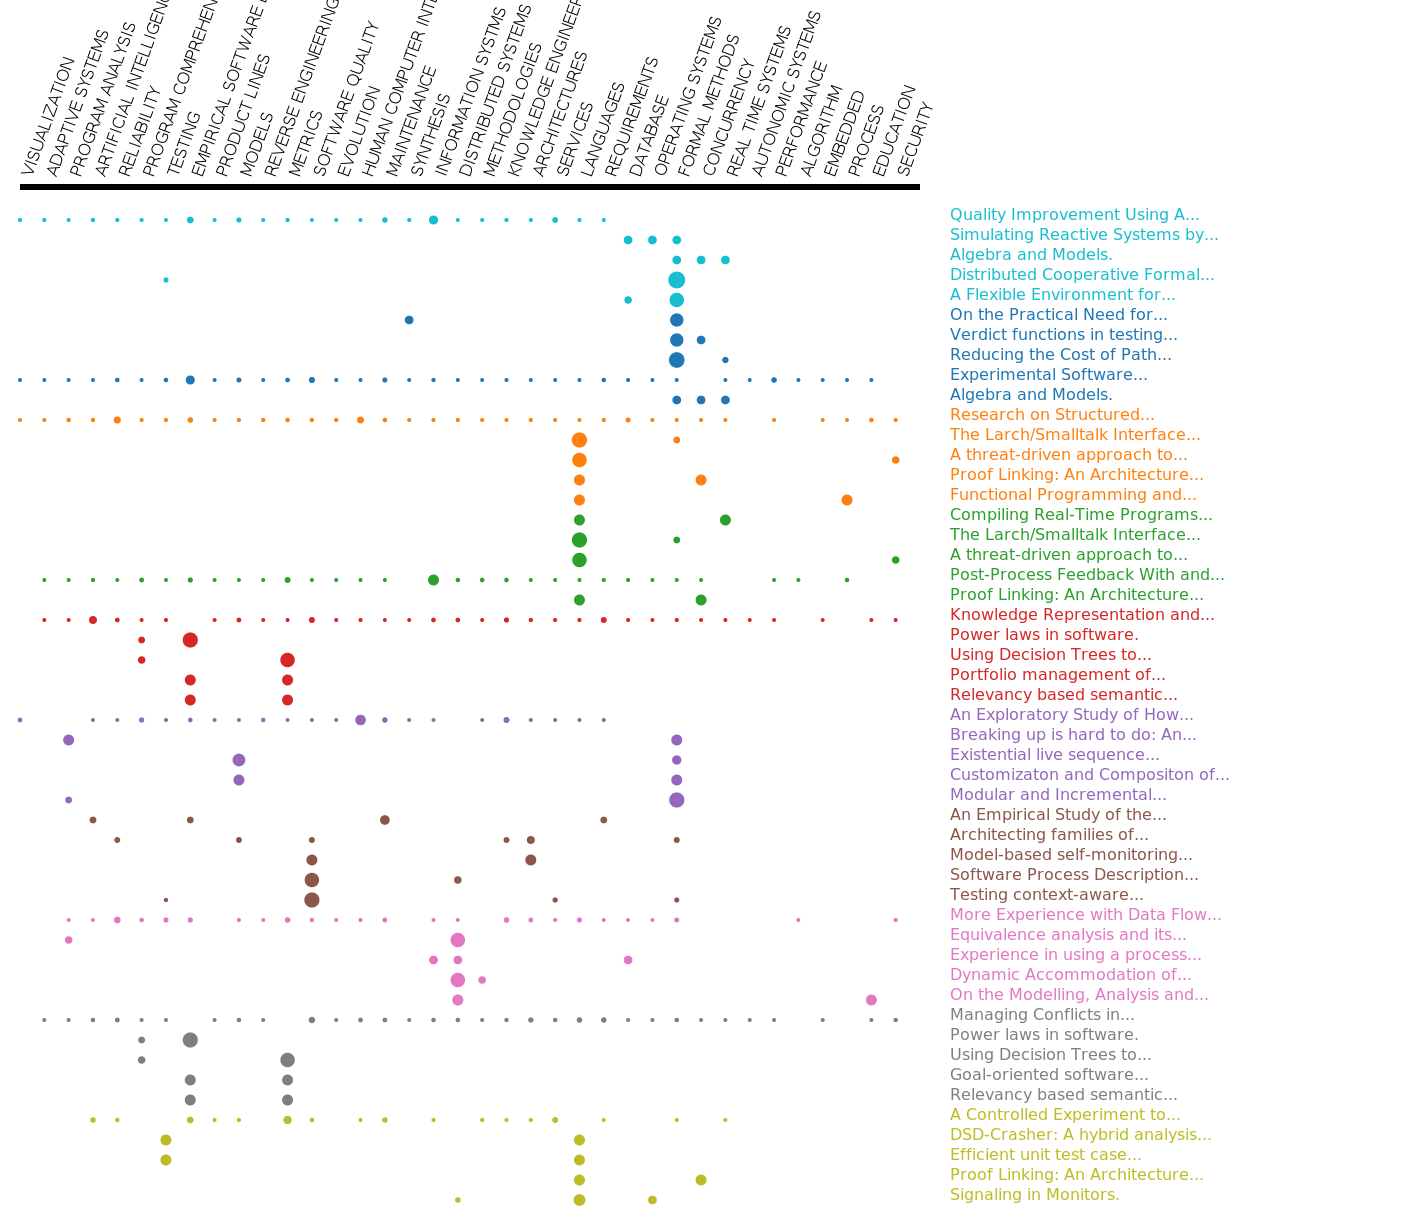
\includegraphics[width=0.45\linewidth]{img/gamma-09-alg-3.png}&
		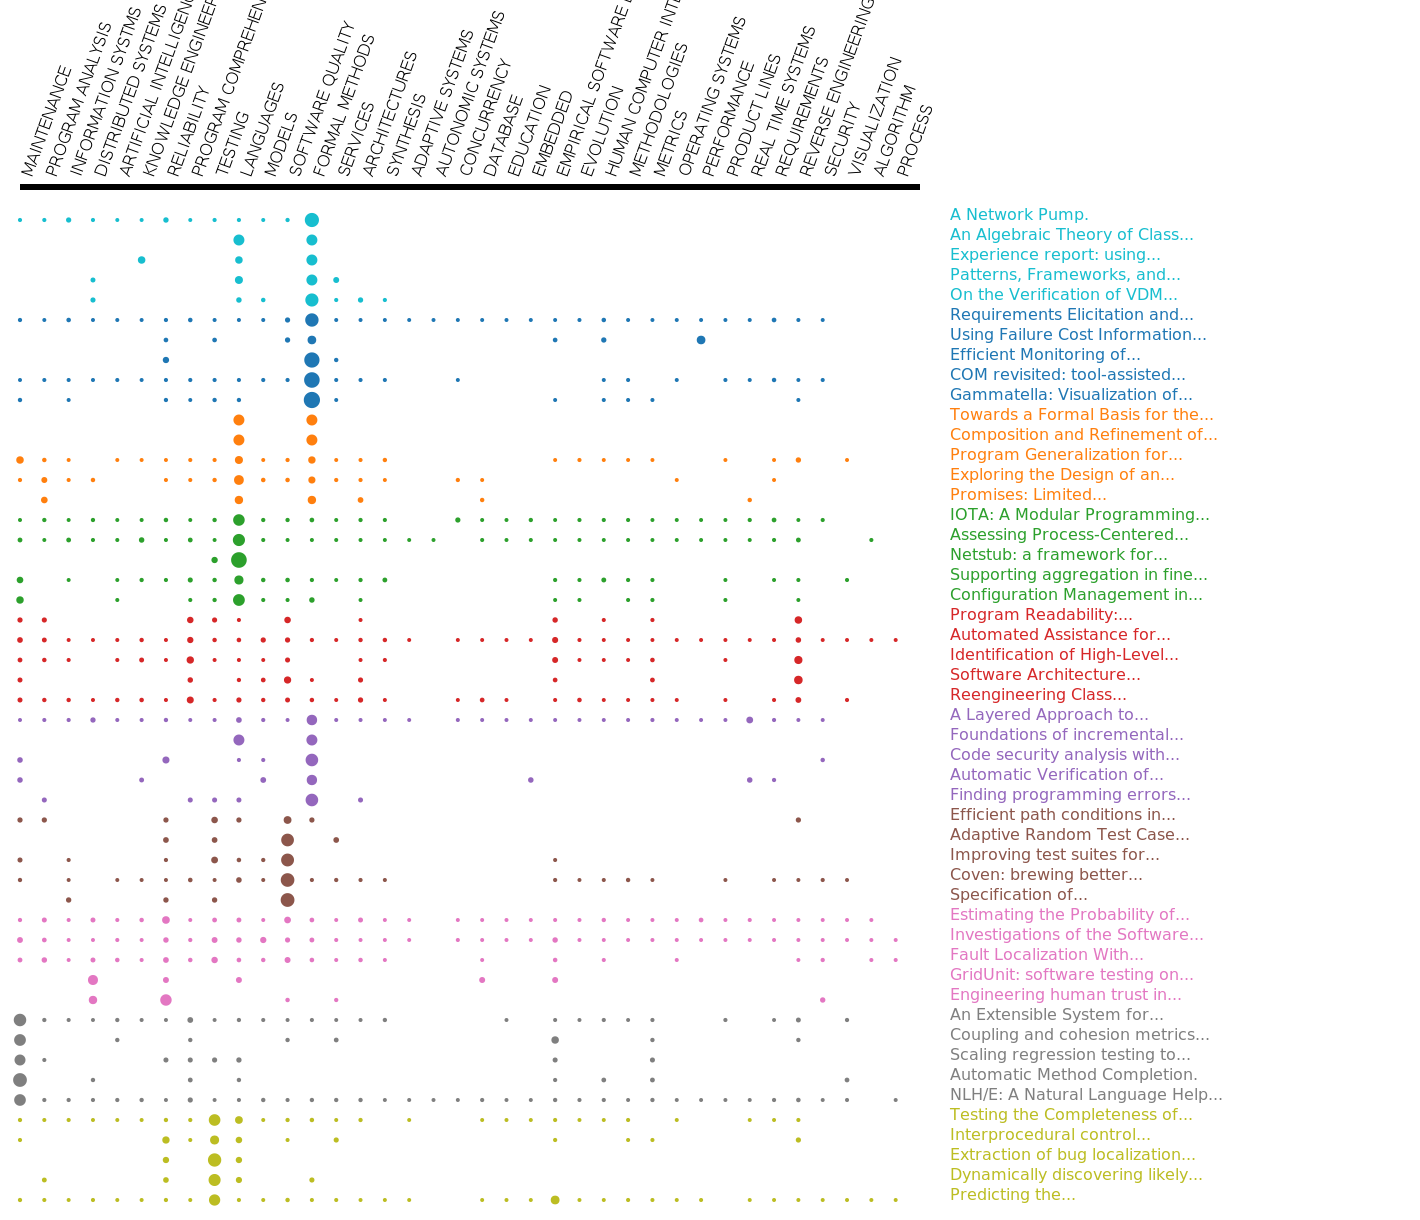
\includegraphics[width=0.45\linewidth]{img/gamma-09-alg-4.png}\\
	\end{tabular}
	\caption{Comparación de soluciones para BOBO-10 con y sin heurística de mejoramiento}
	\label{res:bobo}
\end{figure}

La decisión acerca del valor de $\gamma$ para priorizar un objetivo sobre el otro es realizada por el usuario. Una curva de frontera eficiente podría ayudar para examinar el balance (trade-off) entre los dos objetivos. La intención es que el usuario pueda analizar si una mejora significativa en el valor intra-paquete implica una degradación sustancial en el valor inter-paquetes y viceversa. Para ilustrar este análisis en la Figura \ref{res:inter_intra} se comparan las soluciones obtenidas por los algoritmos $alg1$ y $alg5$ variando en pasos de $0,1$. Una primera evaluación muestra que la mayoría de las soluciones provistas por ambos algoritmos son no dominadas, es decir ninguna solución es mejor en ambos objetivos que cualquier otra solución.

El algoritmo $C-HAC$ de \cite{journals/tkde/Amer-YahiaBCFMZ14} ($alg1$) utiliza la función $Score$ para decidir el par de {\em clusters} a unir en la etapa de producción de paquetes y en la selección simple en la segunda fase. Estos dos criterios omiten la diversidad de los paquetes. De acuerdo a los resultados de la tabla \ref{tabla:comp1}, se pudo concluir que haber considerado la función Intra-Inter y la selección proporcional benefició la calidad de las soluciones cuando la misma es medida a partir de la función objetivo $w(S)$. Con el fin de evaluar que el $alg5$ es capaz de captar efectivamente la diversidad en la solución, se analizaron las soluciones para $\gamma=0.5$. En este caso el $alg1$ obtuvo un valor de $intra=93,82$ y de $inter=35,49$, mientras que el $alg5$ logró valores de $intra=92,94$ y de $inter=35,96$. A pesar de que la solución de $alg1$ es levemente superior, la solución del $alg5$ aumentó el valor $inter$ el $1,32\%$ con un deterioro del valor $intra$ del $0,93\%$. Observando la Figura~\ref{res:inter_intra} se puede ver que la cohesión intra-paquete de ambas soluciones es equivalente. Sin embargo, la diversidad en la segunda solución es mayor, ya que los patrones entre los artículos más similares de distintos paquetes son más heterogéneos. 

En la misma figura se compara las soluciones obtenidas por los algoritmos $alg2$ y el goloso $alg7$. En promedio supera a las soluciones provistas por $alg2$ en $76\%$. De la comparación, se destaca que el valor de $\gamma$ impacta más en las soluciones de $alg2$.  

\begin{figure}[H]
	\centering
	\begin{tabular}{cc}
			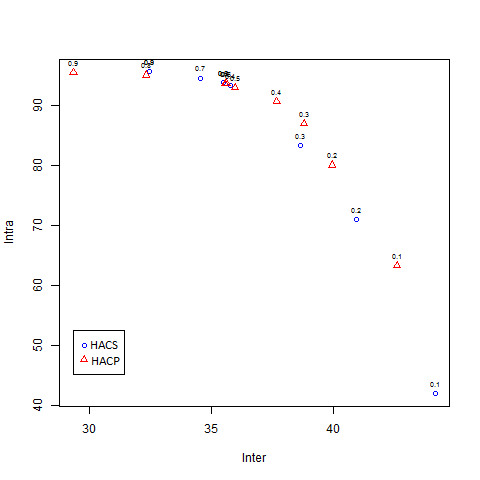
\includegraphics[width=0.45\linewidth]{img/alg1_vs_alg5.png}&
			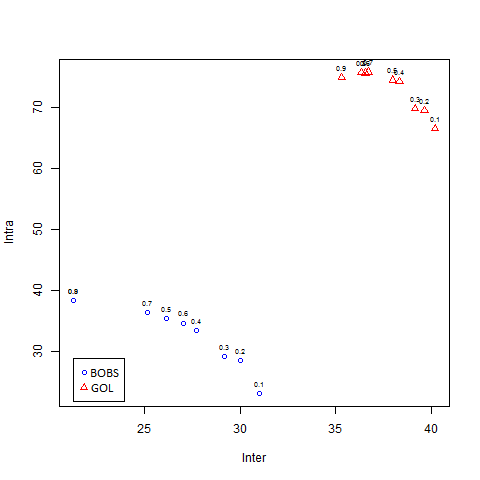
\includegraphics[width=0.45\linewidth]{img/alg2_vs_alg7.png}\\
			$alg1$ vs $alg5$ & $alg2$ vs $alg7$\\
	\end{tabular}
	\caption{Trade-off entre objetivos para los distinos valores de $\gamma$}
	\label{res:inter_intra}
\end{figure}

\subsubsection{Búsqueda de autores}
En la tabla \ref{tabla:comp2} se muestran los porcentajes de deterioro de cada solución con respecto a la mejor solución obtenida para la búsqueda de ``autores que escribieron artículos de tópicos similares que están afiliados a distintas universidades''. Se observa que en este caso, a diferencia de la búsqueda de artículos, el algoritmo tabú halló en todos los casos la mejor solución. Con la particularidad que el algoritmo goloso tuvo muy poco deterioro con respecto a la mejor solución, alcanzando en algunos casos el mismo valor de función objetivo.

Los algoritmos jerárquicos $C-HAC$ e $Inter-Intra C-HAC$ siguen demostrando que obtienen las mejores soluciones en comparación a $BOBO$, sobre todo $alg6$ que contiene la búsqueda tabú. Éstas búsquedas vuelven a indicar que las soluciones pueden ser mejoradas en porcentajes muy significativos. Como ocurrió en el caso del algoritmo $alg3$, mejorando las soluciones en un promedio cercano al $30\%$ y también para $alg5$ y $alg7$ que en todos los casos mejoraron sus valores iniciales. Con respecto a la estrategia de selección proporcional aplicada al algoritmo $BOBO$ no se observaron mejoras, aunque las soluciones obtenidas fueron cercanas en términos de función objetivo. 

\begin{table}[H]
\begin{center}
\begin{tabular}{|c|c|c|c|c|c|c|c|c|}
\hline
$\gamma$&$alg1$&$alg2$&$alg3$&$alg4$&$alg5$&$alg6$&$alg7$&$alg8$ \\ \hline
0.1 & -0.33 & -21.59 & -26.05 & -1.74 & -0.13 & 0.00 & -0.61 & 0.00 \\
0.2 & -0.63 & -27.46 & -29.71 & -0.52 & -0.36 & 0.00 & -1.10 & -0.25 \\
0.3 & -0.44 & -30.57 & -32.47 & -0.20 & -0.53 & 0.00 & -1.50 & -0.34 \\
0.4 & -0.25 & -32.63 & -34.29 & -0.32 & -0.25 & 0.00 & -1.88 & -0.73 \\
0.5 & -0.22 & -34.42 & -35.84 & -0.04 & 0.00 & 0.00 & -2.15 & -0.79 \\
0.6 & -0.18 & -35.86 & -37.05 & -2.01 & 0.00 & 0.00 & -2.45 & -1.39 \\
0.7 & 0.00 & -37.10 & -37.93 & -1.71 & -0.12 & 0.00 & -2.59 & -0.96 \\ 
0.8 & 0.00 & -38.19 & -38.70 & -1.44 & -0.08 & 0.00 & -2.72 & -1.20 \\
0.9 & -0.03 & -39.15 & -39.38 & -1.21 & -0.10 & 0.00 & -3.35 & -1.72 \\ \hline 
\end{tabular}
\caption{Comparación de calidad de soluciones entre algoritmos para la \hyperref[busqueda:autores]{búsqueda de autores}} 
\label{tabla:comp2}
\end{center}
\end{table}

Para analizar el trade-off entre la parte inter y la intra en la figura \ref{res:aut_alg1_vs_alg5_vs_alg7} del lado izquierdo se muestra los valores inter e intra de las soluciones obtenidas por los algoritmos $alg1$, $alg2$, $alg5$ y $alg7$ para todos los $\gamma$. Puede apreciarse, como es de esperar, que los valores del $alg2$ son significativamente inferiores al resto de los algoritmos. En cambio los valores de $alg1$, $alg5$ y $alg7$ se concentran en una región reducida, ya que sus soluciones fueron muy similares respecto al valor de la función objetivo.

A la derecha de la figura \ref{res:aut_alg1_vs_alg5_vs_alg7} se encuentran los valores inter e intra de los algoritmos $alg1$ y $alg5$. Puede verse como los valores de las soluciones obtenidas con $alg5$ no están dominadas por la parte inter y si más concentradas en la parte intra, a diferencia de los que ocurre con $alg1$.

\begin{figure}[H]
	\centering
	\begin{tabular}{cc}
			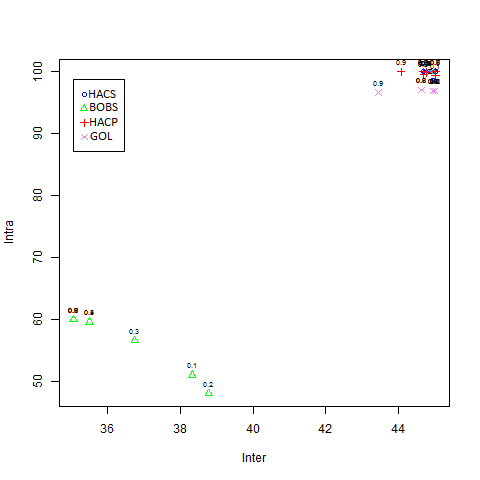
\includegraphics[width=0.45\linewidth]{img/aut-alg1-alg2-alg5-alg7.png}&
			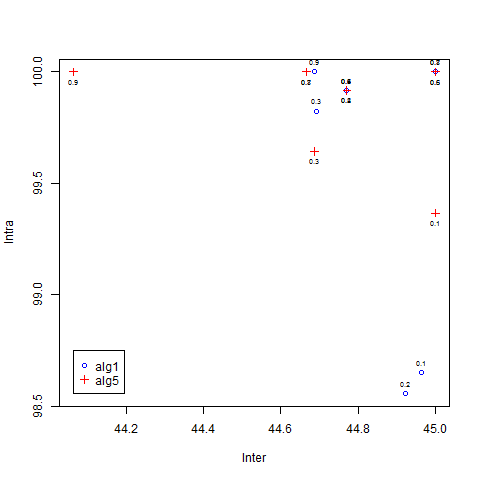
\includegraphics[width=0.45\linewidth]{img/aut-alg1-alg5.png}\\
	\end{tabular}
	\caption{}
	\label{res:aut_alg1_vs_alg5_vs_alg7}
\end{figure}


En la figura \ref{res:aut-alg-6} de la solución generada por el algoritmo $alg6$ para $\gamma = 0.1$, se tienen las siguientes observaciones:
\begin{enumerate}
	\item Todos los paquetes contienen autores que pertenecen a los mismos tópicos. 
	\item No existe un tópico que esté presente en más de un paquete.
	\item Todos los paquetes utilizan el máximo del presupuesto.
\end{enumerate}
Por (1) y (2) la calidad intra e inter paquete es máxima respectivamente. Con (3) se cumple que la solución obtenida es la de máxima calidad para todo $\gamma$. Para todas las búsquedas realizadas, las soluciones que se obtuvieron cumplían con las observaciones mencionadas.

\begin{figure}[H]
  \centering
    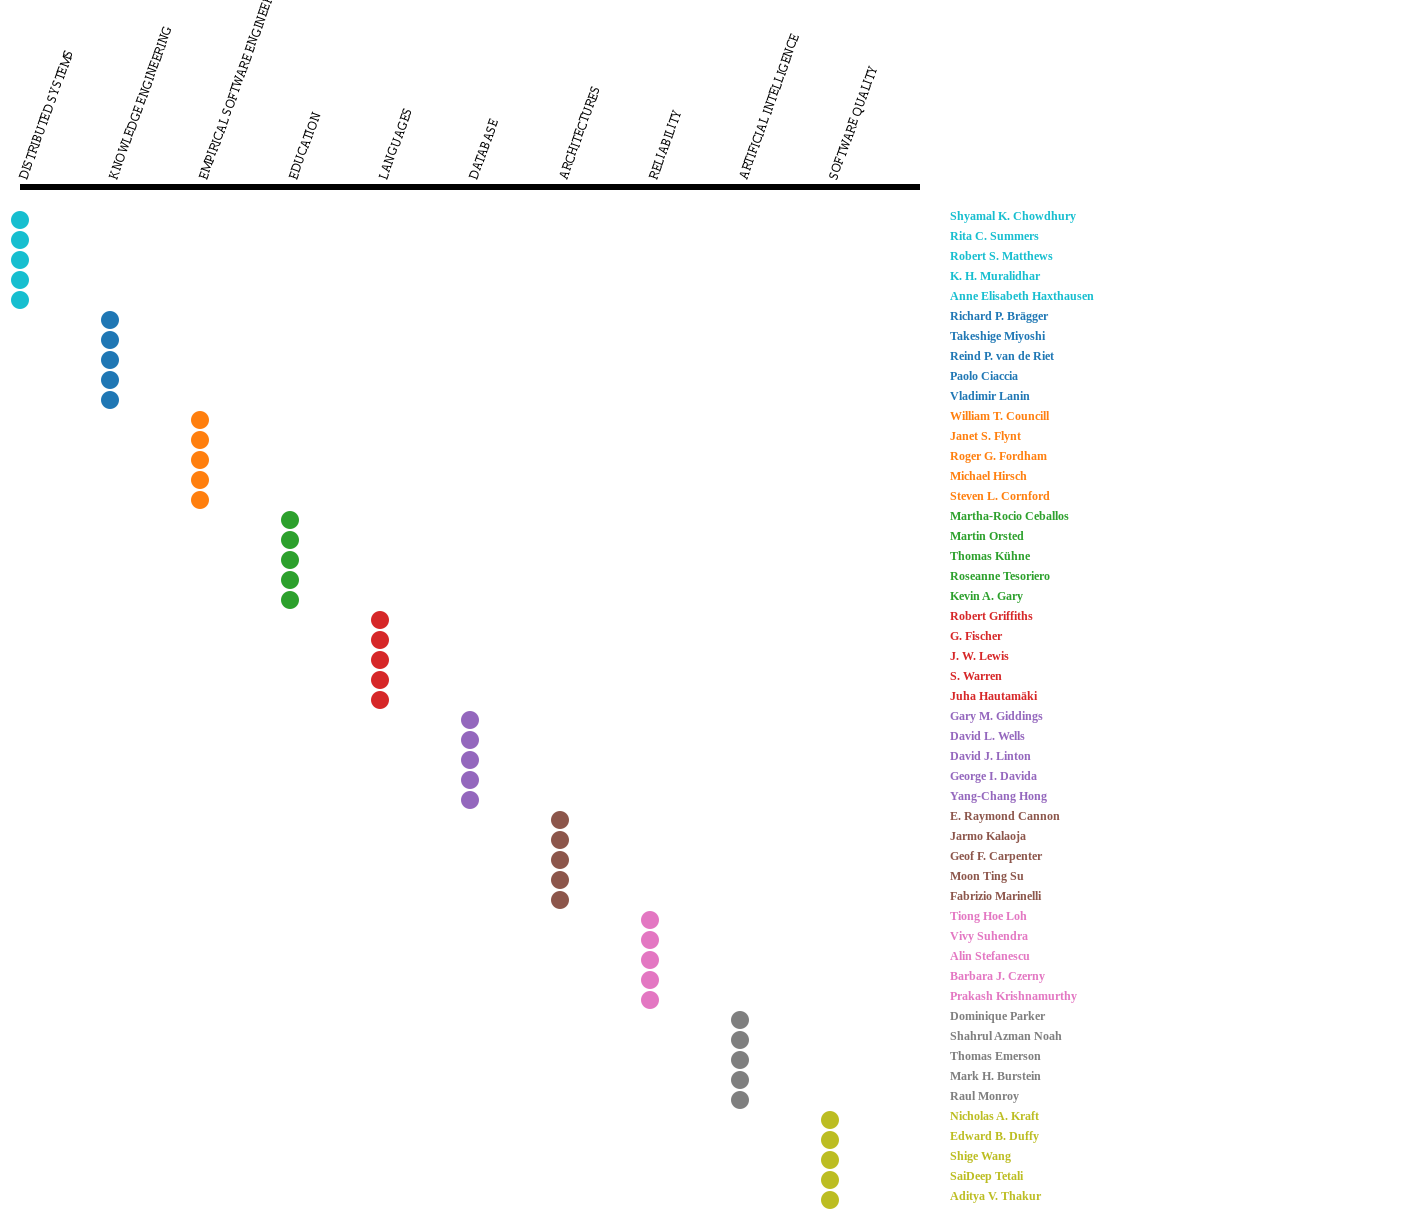
\includegraphics[width=1\textwidth]{img/aut-alg-6.png}
  \caption{}
  \label{res:aut-alg-6}
\end{figure}



\subsubsection{Búsqueda de universidades}
En este escenario lo que más se destaca de la tabla \ref{tabla:comp3} es el comportamiento del algoritmo $alg1$ que generó una mejor solución para los valores de $\gamma\ =\ 0.1$ y $\gamma\ =\ 0.2$ con respecto al algoritmo $alg6$. En el resto de las soluciones obtenidas (de $alg1$ y $alg6$) se aprecia un deterioro cada vez más significativo a medida que crece el valor del $\gamma$.

Por otro lado la función objetivo de las soluciones provista por los algoritmos $alg2$, $alg3$ y $alg7$ se encuentran muy alejadas de las soluciones provistas por los jerárquicos. En el caso del algoritmo goloso $alg7$ las soluciones mejoran con respecto a los algoritmos $alg2$ y $alg3$ cuando el valor de $\gamma$ disminuye.

Al igual que en el resto, la búsqueda tabú mejoró las soluciones iniciales del $BOBO$ y del algoritmo goloso considerablemente. Se destaca que para las soluciones jerárquicas la búsqueda tabú siempre mejora la solución inicial sin importar que tan buena sea.
\begin{table}[H]
\begin{center}
\begin{tabular}{|c|c|c|c|c|c|c|c|c|}
\hline
$\gamma$&$alg1$&$alg2$&$alg3$&$alg4$&$alg5$&$alg6$&$alg7$&$alg8$ \\ \hline
0.1 & 0.00 & -30.89 & -31.26 & -15.05 & -1.39 & -1.33 & -10.97 & -9.73 \\
0.2 & 0.00 & -40.35 & -40.16 & -22.09 & -1.72 & -1.07 & -22.83 & -20.42 \\
0.3 & -2.22 & -50.85 & -49.98 & -27.01 & -2.37 & 0.00 & -36.06 & -28.55 \\
0.4 & -5.72 & -60.65 & -58.96 & -33.76 & -1.36 & 0.00 & -48.44 & -30.38 \\
0.5 & -8.59 & -69.76 & -67.66 & -31.46 & -1.92 & 0.00 & -60.18 & -34.32 \\
0.6 & -12.09 & -77.50 & -74.71 & -33.85 & -2.53 & 0.00 & -70.16 & -35.80 \\
0.7 & -12.59 & -82.97 & -80.09 & -31.52 & 0.00 & 0.00 & -78.04 & -29.36 \\
0.8 & -15.52 & -88.12 & -84.93 & -32.90 & 0.00 & 0.00 & -85.63 & -36.34 \\
0.9 & -17.46 & -88.10 & -87.79 & -31.16 & 0.00 & 0.00 & -92.13 & -28.26 \\
 \hline 
\end{tabular}
\caption{Comparación de calidad de soluciones entre algoritmos para la \hyperref[busqueda:universidades]{búsqueda de universidades}} 
\label{tabla:comp3}
\end{center}
\end{table}

\subsection{Análisis de los resultados obtenidos de la base de datos de atracciones turísticas}\label{res:busAtracciones}
En las búsquedas realizadas sobre la base de datos de atracciones turísticas las soluciones obtenidas a partir de las modificaciones propuestas en este trabajo de los algoritmos PAC, como puede observarse en la tabla \ref{tabla:comp4}, mejoran a los originales en todos los casos. Es para destacar que en este escenario el algoritmo goloso supera a $alg1$. La búsqueda tabú consiguió mejores resultados para los algoritmos PAC. Por otro lado en el algoritmo goloso, en contraste a lo sucedido en las demás consultas, la heurística de búsqueda no obtuvo mejores soluciones.

\begin{table}[H]
\begin{center}
\begin{tabular}{|c|c|c|c|c|c|c|c|c|}
\hline
$\gamma$&$alg1$&$alg2$&$alg3$&$alg4$&$alg5$&$alg6$&$alg7$&$alg8$ \\ \hline
0.1 & -6.49 & -22.89 & -22.30 & -9.99 & -0.05 & 0.00 & -0.52 & -0.52 \\
0.2 & -13.50 & -27.60 & -26.57 & -16.51 & -0.09 & 0.00 & -1.09 & -1.09 \\
0.3 & -21.10 & -32.76 & -29.73 & -20.58 & -0.15 & 0.00 & -1.70 & -1.70 \\
0.4 & -29.38 & -36.68 & -33.51 & -25.10 & -0.20 & 0.00 & -2.37 & -2.37 \\
0.5 & -38.43 & -42.05 & -38.44 & -30.94 & -0.27 & 0.00 & -3.10 & -3.10 \\
0.6 & -48.35 & -47.73 & -43.86 & -34.75 & -0.34 & 0.00 & -3.90 & -3.90 \\
0.7 & -59.29 & -51.47 & -50.54 & -43.46 & -0.41 & 0.00 & -4.78 & -4.78 \\
0.8 & -71.36 & -57.07 & -56.14 & -45.61 & 0.00 & 0.00 & -5.62 & -5.62 \\
0.9 & -84.97 & -60.59 & -59.81 & -44.04 & 0.00 & 0.00 & -7.33 & -7.33 \\
\hline 
\end{tabular}
\caption{Comparación de calidad de soluciones entre algoritmos para la \hyperref[busqueda:atracciones]{búsqueda de atracciones turísticas}}
\label{tabla:comp4}
\end{center}
\end{table}

\subsection{Análisis general de los resultados obtenidos}
Se obtuvieron mejores resultados en términos de los valores de la función objetivo, así como en la sensibilidad al criterio de valorización de cada objetivo sin perjuicio en el tiempo de ejecución. En el caso de los algoritmos $PAC$ usando generación de paquetes mediante las técnicas $BOBO$ y aplicando la búsqueda tabú el resultado mejoró considerablemente, como puede verse en \autoref{tabla:comp1} y \autoref{tabla:comp2}.

Se observó que las soluciones obtenidas utilizando el algoritmo goloso fueron mejores en comparación a las generadas por la metodología $PAC$, solo cuando en la etapa de producción se utilizó la estrategia $BOBO$. Por el contrario, la producción jerárquica derivó en la obtención final de mejores paquetes. Si bien la técnica de las implementaciones de $BOBO$ son golosas, éstas solo hacen hincapié en los valores intra de la función objetivo. Mientras qué la nueva propuesta lo hace sobre la totalidad de la función objetivo. 

Para la estrategia PAC las implementaciones de BOBO fueron en todos los casos las más rápidas, resultando ser las ideales para instancias de tamaño muy grandes. La solución obtenida mejorá considerablemente si se le aplica la búsqueda tabú. En las pruebas realizadas con HAC con un universo de elementos menor a los 10000 se cuadruplican o quintuplican los tiempos de ejecución debido a su complejidad ($\mathcal{O}(N^{2}\log n)$). Sin embargo en instancias más chicas como las atracciones turísticas los tiempos fueron muy cercanos entre ellos.

Las soluciones obtenidas usando \texttt{Efficient-HAC} y búsquedas golosas para valores de $\gamma$ menores a $0.5$ fueron \textquotedblleft similarmente buenas\textquotedblright , dado que los resultados en términos de función objetivo fueron cercanos. En cambio para $\gamma$ más cercanos a uno se observó que el valor de la función objetivo de las soluciones HAC resultaron significativamente mayores. En todos los casos se identificó que las relaciones inter-paquetes son mejores en las soluciones del algoritmo goloso, logrando soluciones más interdependientes.

Al comparar \texttt{BOBO-10} y \texttt{BOBO-160} usando la selección simple se observa que la diferencia entre los valores de la función objetivo de cada solución aumenta a medida que $\gamma$ se acerca a $1$. Se supone que esto se debe a la estrategia \texttt{produce and choose}. El objetivo de la primera etapa es producir paquetes con máximo valor de similitud. En el caso de que se requiera una solución con mayor separación entre paquetes, al haber producido menos cantidad de paquetes existen menos posibilidades para generar una solución más dispersa. Un mismo análisis se podría hacer si se compara \texttt{BOBO-10} y \texttt{HAC}.

Comparando los resultados obtenidos al realizar la selección de a un candidato contra la selección de a pares se obtuvo que para \texttt{BOBO-160} y \texttt{HAC} los tiempos aumentaron a $40$ minutos y para \texttt{BOBO-10} a $2$ minutos. En cuanto al valor de la función objetivo el único beneficiado fue \texttt{BOBO-10} ya que para \texttt{HAC} empeoró y para \texttt{BOBO-160} el aumento fue muy pequeño en comparación al incremento de tiempo.
\chapter{Conclusiones}
\label{chap:conclusiones}
\section{Comparaciones entre los diferentes algoritmos}\label{conc:compDifAlgo}
\subsection{Papers}
Con los resultados obtenidos podemos hacer dos tipos de análisis y comparaciones, la primera y más 
clara es comparar entre los algoritmos \texttt{SingleHAC} y \texttt{EfficientHAC}, en la que 
observamos que para $\gamma$ bajos obtuvimos los mismos resultados, pero para $\gamma$ altos a 
partir de $0.7$ obtuvimos soluciones diferentes las cuáles tenían un valor con respecto a la 
función objetivo prácticamente iguales pero se obtuvieron mejores relaciones interbundles.\\
La otra comparación que surge es entre \texttt{EfficientHAC} y \texttt{Greedy} en el que se observa 
que para $\gamma$ las soluciones obtenidas son \textquotedblleft similarmente 
buenas\textquotedblright , dado que sus valores en términos de función objetivo están cercanos, 
pero a la vez observamos que la relación interbundles es mejor las soluciones de la implementación 
\texttt{Greedy}. En cambio para $\gamma$ altos, el valor de la función objetivo en la 
implementación \texttt{EfficientHAC} fue muy superior pero la relación interbundles en el algoritmo 
\texttt{Greedy} se ve que fue mejor, logrando soluciones mas interdependientes.

\section{Valores cercanos al óptimo}
Dada la función que se está intentando maximizar $$\displaystyle\sum_{1 \leq i \leq k} 
\displaystyle\sum_{u,v \in S_{i}} \gamma s(u,v)\ 
+\ \displaystyle\sum_{1 \leq i \leq j \leq k} (1-\gamma) (1 - \displaystyle\max_{u \in S_{1}, v 
\in S_{j}} s(u,v))$$ podemos hacer suposiciones para ver que tan lejos o cerca están de algunas de 
los valores óptimos según el $\gamma$.\\
Para las siguientes cotas supongamos escenarios ideales en el cuál la soluciones contiene bundles 
donde todos sus elementos tienen una similitud máxima (igual a 1) y los bundles entre si son 
completamente diferentes, o sea, la similitud entre cada bundle es 0. Con estas hipótesis podemos 
ver que la reemplazar la función por $$\displaystyle\sum_{1 \leq i \leq k} 
\displaystyle\sum_{u,v \in S_{i}} \gamma 1\ 
+\ \displaystyle\sum_{1 \leq i \leq j \leq k} (1-\gamma) (1 - \displaystyle\max_{u \in S_{1}, v 
\in S_{j}} 0)$$ que luego se transforma en $$\displaystyle\sum_{1 \leq i \leq k} 
\displaystyle\sum_{u,v \in S_{i}} \gamma 1\ 
+\ \displaystyle\sum_{1 \leq i \leq j \leq k} (1-\gamma) 1$$ como en nuestro caso $k\ =\ 10$ y la 
cantidad de items por bundle es $5$ entonces la sumatoria se resume en $$\displaystyle\gamma\ 100\ 
+\ (1-\gamma)\ 45$$
Para los $\gamma \in (0.1, 0.3, 0.5, 0.7, 0.9)$ los resultados de la función son los siguientes:\\
\begin{table}[H]
  \centering
  \resizebox{0.5\textwidth}{!} {
    \begin{tabular}{|lc|}
    \hline
    $\gamma$ & Valor función objetivo \\
    \hline
    $0.1$  & $50.5$ \\
    $0.3$  & $61.5$ \\
    $0.5$  & $72.5$ \\
    $0.7$  & $83.5$ \\
    $0.9$  & $94.5$ \\
    \hline
    \end{tabular}
  }
    \caption {Valor óptimo de la función para cada $\gamma$}
\end{table}

En las ejecuciones del algoritmo \textbf{SingleHAC} para artículos en los $\gamma$ más altos los 
resultados de los bundles eran los mismos lo cuál se explica porque a medida que $\gamma$ aumenta se 
acerca cada vez más a la cota superior que establecimos. No sucediendo los mismo con $\gamma$ 
menores.\\
En cambio para las ejecuciones también del algoritmo \textbf{SingleHAC} pero para autores en todas 
las soluciones obtuvimos los mismos bundles y se ve reflejado porque la función objetivo para cada 
$\gamma$ es igual a la cota.

%\chapter{Implementación}
%\section{Cálculo de la similitud}
Previo a la ejecución de los algoritmos de búsquedas realizamos los cálculos entre todos los elementos involucrados, papers ya autores. Lo realizamos de esta manera con el objetivo de optimizar los tiempos de ejecución de las búsquedas ya que en cada paso cuando tiene que comparar dos items no necesita calcular el $\cos(\theta)$ de los vectores de sus perfiles y en cambio solo accede a una posición de una matriz que mantenemos en memoria.\\
Si bien de esta manera ganamos en tiempo de ejecución, lo que perdemos es la complejidad espacial ya que estamos manteniendo una matriz de entre $8$ y $22$ millones de registros. En nuestro caso al contar con instancias de no mas de $7000$ elementos no es un problema porque en ningún momento alcanza a pasar los $4$ GB de memoria, lo cuál encontramos en cualquier pc medianamente moderna.
\chapter{Trabajo futuro}
\label{chap:trabajos-futuros}
\section{Desarrollo}
\begin{itemize}
 \item Mejorar las búsquedas tabú para encontrar mejores soluciones.
 \item Nuevas heurísticas para intentar mejorar las soluciones.
\end{itemize}


\section{User friendly}
\begin{itemize}
 \item Generar una interfaz de usuario amgigable.
 \item Una mejor manera de visualizar los resultados de manera on line.
\end{itemize}

\section{Performance}
\begin{itemize}
 \item Acelerar los tiempos de ejecución.
 \item Depuración del código.
 \item Ejecución en diferentes hilos.
 \item Tunning de la base de datos.
\end{itemize}

\section{Extensibilidad}
\begin{itemize}
 \item Generar una interfaz genérica para poder trabajar con datos de cualquier origen y poder ser explotados de la misma forma.
 \item Adaptar el código para poder lograr 
\end{itemize}

%\chapter{Apéndice}
%\section{Resultados de las ejecuciones de los algoritmos de búsqueda}
A continuación se muestra el valor de la función objetivo para cada uno de los distintos algoritmos ejecutados y el tiempo de ejecución final.
\subsection{Artículos}
\Solucion
{}
{simple, por tuplas y proporcional}
{\texttt{HAC} y \texttt{BOBO-x}, con  $x \in$ $(10, 160)$}
{$\in$ $(0,1; 0,3; 0,5; 0,7; 0,9)$}
{10}
{5}
A continuación se muestran los valores de la función objetivo obtenidos:\\
\begin{table}[H]
\centering
  \resizebox{\textwidth}{!} {
    \begin{tabular}{|lc|cccc|}
    \hline
    ~  & ~ & \multicolumn{2}{|c}{Valor función objetivo} & \multicolumn{2}{c|}{Duración de la 
ejecución (mm:ss)} \\
    Algoritmo & gamma & Selección simple & Selección proporcional & Selección simple          
         & Selección proporcional \\ 
    \hline
    HAC & $0,1$ & $48,9470$  & $35,1979$ & $10:00$ & $40:00$ \\
    HAC & $0,3$ & $59,1852$  & $58,7049$ & $10:00$ & $40:00$ \\
    HAC & $0,5$ & $70,5931$  & $70,205$ & $10:00$ & $40:00$ \\
    HAC & $0,7$ & $82,0687$  & $81,8331$ & $10:00$ & $40:00$ \\
    HAC & $0,9$ & $93,8227$  & $93,7189$ & $10:00$ & $40:00$ \\
    BOBO-160 & $0,1$ & $33,3762$  & $35,1979$ & $6:00$ & $46:00$ \\
    BOBO-160 & $0,3$ & $33,2741$  & $34,4164$ & $6:00$ & $46:00$ \\
    BOBO-160 & $0,5$ & $37,3484$  & $37,0669$ & $6:00$ & $46:00$ \\
    BOBO-160 & $0,7$ & $40,4186$  & $40,1762$ & $6:00$ & $46:00$ \\
    BOBO-160 & $0,9$ & $49,0972$  & $44,9824$ & $6:00$ & $46:00$ \\
    BOBO-10 & $0,1$ & $29,3038$  & $30,5376$ & $1:30$ & $2:00$ \\
    BOBO-10 & $0,3$ & $25,9363$  & $26,6800$ & $1:30$ & $2:00$ \\
    BOBO-10 & $0,5$ & $20,9841$  & $22,9482$ & $1:30$ & $2:00$ \\
    BOBO-10 & $0,7$ & $22,3052$  & $23,2333$ & $1:30$ & $2:00$ \\
    BOBO-10 & $0,9$ & $18,8381$  & $21,9347$ & $1:30$ & $2:00$ \\
    BOBO-ex & $0,1$ & $35,5786$  & - & $14:00$ & - \\
    BOBO-ex & $0,3$ & $35,4117$  & - & $14:00$ & - \\
    BOBO-ex & $0,5$ & $39,4408$  & - & $14:00$ & - \\
    BOBO-ex & $0,7$ & $45,0940$  & - & $14:00$ & - \\
    BOBO-ex & $0,9$ & $51,2695$  & - & $14:00$ & - \\
    \hline
    \end{tabular}
  }
  \caption {Valor función objetivo y tiempo de ejecución para la búsqueda de artículos similares}
\end{table}
\subsection{Autores}
\Solucion
{}
{simple y proporcional}
{\texttt{HAC} y \texttt{BOBO-x}, con  $x \in$ $(10, 160)$ y \texttt{BOBO-ex}}
{$\in$ $(0,1; 0,3; 0,5; 0,7; 0,9)$}
{10 y 20}
{5 y 10}
\begin{table}[H]
\centering
  \resizebox{\textwidth}{!} {
    \begin{tabular}{|lc|cccc|}
    \hline
    ~  & ~ & \multicolumn{2}{|c}{Valor función objetivo} & \multicolumn{2}{c|}{Duración de la 
ejecución (mm:ss)} \\
    Algoritmo & gamma & Selección simple & Selección proporcional & Selección simple          
         & Selección proporcional \\ 
    \hline
    HAC & $0,1$ & $50,5$  & $50,5$ & $8:40$ & $9:00$ \\
    HAC & $0,3$ & $61,5$  & $61,5$ & $8:40$ & $9:00$ \\
    HAC & $0,5$ & $72,5$  & $72,5$ & $8:40$ & $9:00$ \\
    HAC & $0,7$ & $83,5$  & $83,5$ & $8:40$ & $9:00$ \\
    HAC & $0,9$ & $94,5$  & $94,5$ & $8:40$ & $9:00$ \\
    BOBO-160 & $0,1$ & $38,6883$  & $36,8917$ & $10:00$ & $8:00$ \\
    BOBO-160 & $0,3$ & $43,4380$  & $41,4767$ & $10:00$ & $8:00$ \\
    BOBO-160 & $0,5$ & $47,3612$  & $47,9337$ & $10:00$ & $8:00$ \\
    BOBO-160 & $0,7$ & $51,5712$  & $52,1462$ & $10:00$ & $8:00$ \\
    BOBO-160 & $0,9$ & $57,2009$  & $57,5260$ & $10:00$ & $8:00$ \\
    BOBO-10 & $0,1$ & $30,2956$  & $31,6080$ & $2:30$ & $2:30$ \\
    BOBO-10 & $0,3$ & $33,6794$  & $35,4411$ & $2:30$ & $2:30$ \\
    BOBO-10 & $0,5$ & $33,0506$  & $37,5776$ & $2:30$ & $2:30$ \\
    BOBO-10 & $0,7$ & $37,2855$  & $34,5657$ & $2:30$ & $2:30$ \\
    BOBO-10 & $0,9$ & $41,0119$  & $35,2511$ & $2:30$ & $2:30$ \\
    BOBO-ex & $0,1$ & $39,9767$  & $39,9767$ & $27:00$ & $27:00$ \\
    BOBO-ex & $0,3$ & $44,0043$  & $44,0043$ & $27:00$ & $27:00$ \\
    BOBO-ex & $0,5$ & $48,5481$  & $48,5481$ & $27:00$ & $27:00$ \\
    BOBO-ex & $0,7$ & $53,1993$  & $53,1993$ & $27:00$ & $27:00$ \\
    BOBO-ex & $0,9$ & $57,7400$  & $57,7400$ & $27:00$ & $27:00$ \\
    \hline
    \end{tabular}
  }
  \caption {Valor función objetivo y tiempo de ejecución para la búsqueda de autores similares}
\end{table}



%%%% BIBLIOGRAFIA
\backmatter
\bibliographystyle{plain}
\bibliography{tesis} 

\end{document}
